%\documentclass[pdf,final,colorBG,slideColor]{prosper}
\documentclass[xcolor=dvipsnames]{beamer}
%%\usetheme{default}
\usecolortheme[named=Maroon]{structure}
%\usetheme{Boadilla}
\usetheme{Madrid}
\useoutertheme{default}%[footline=empty]{infolines}

% \usepackage{helvet}
% \usepackage{enumerate}
% \usepackage{amsmath}
% \usepackage{amsfonts}
% \usepackage{graphicx}
% \usepackage{ulem}
% \usepackage{multirow}
\usepackage{comment}
\usepackage{xspace}

\usepackage[absolute,overlay]{textpos}
\usepackage[ruled]{./algorithm2e}
%%for algorithm2e package, label has to be following caption in the same line!!!
\renewcommand{\algorithmcfname}{ALGORITHM}
\SetAlFnt{\small}
\SetAlCapFnt{\small}
\SetAlCapNameFnt{\small}
\SetAlCapHSkip{0pt}
\IncMargin{-\parindent}

%\RequirePackage{algorithmic}
%\RequirePackage{algorithm}
% \renewcommand{\algorithmicrequire}{\textbf{Inputs:}}
% \renewcommand{\algorithmicensure}{\textbf{Outputs:}}


%\newtheorem{theorem}{Theorem}
%\newtheorem{lemma}{lemma}
%\newtheorem{corollary}{Corollary}
%\newtheorem{proposition}{Proposition}
%\newtheorem{Q}{Question}
%\newtheorem{Exa}{Example}
%\newtheorem{Definition}{Definition}


\newcommand{\Fq}{{\mathbb{F}}_{q}}
\newcommand{\Fkk}{{\mathbb{F}}_{2^k}}
\newcommand{\Zkk}{{\mathbb{Z}}_{2^k}}
\newcommand{\Fkkx}[1][x]{\ensuremath{\mathbb{F}}_{2^k}[#1]\xspace}
\newcommand{\Grobner}{Gr\"{o}bner\xspace}
%\newcommand{\Grobner}{Gr\"{o}bner}
\newcommand{\bi}{\begin{itemize}}
\newcommand{\ei}{\end{itemize}}
\newcommand{\F}{{\mathcal{F}}}
\newcommand{\B}{{\mathbb{B}}}


\title[GF Abstraction using \Grobner Bases]{Word-Level Polynomial Abstraction From Circuits Using \Grobner Bases}

\author[Tim Pruss]{Tim Pruss}

%\email{rostamian@umbc.edu}
\institute[Univ. of Utah]{
%\includegraphics[height=17mm]{/Users/Kalla/teaching/Comp-Algebra-Course/lectures/old_ulogo.eps}\\
Graduate Student\\
Electrical and Computer Engineering, University of Utah\\
pruss.tim@gmail.com\\
\ \\
\ \\
{\bf Master's Thesis Proposal}\\
}


\date{}
%\slideCaption{}

%% Images
%\pgfdeclareimage[width=.4in]{fg:logo}{/Users/Kalla/teaching/Comp-Algebra-Course/lectures/old_ulogo.eps} 

%%%%%%%%%%%%%%%%%%%%%%%%%%%%%%%%%%%%%%%%%%%%%%%%%%
%%%%%%%%%%%%%%%%%%%%%%%%%%%%%%%%%%%%%%%%%%%%%%%%%%
%%%%%%%%%%%%%%%%%%%%%%%%%%%%%%%%%%%%%%%%%%%%%%%%%%
\begin{document}


%----------- titlepage ----------------------------------------------%
\begin{frame}[plain]
  \titlepage

\end{frame}

%\maketitle

%%%%%%%%%%%%Try section
% \section*{Outline}
% \begin{frame}

% \tableofcontents
% \end{frame}

% \section{Intro}
% \subsection{What's that?}
% \subsection{Overview of something}

% \section{Galois Fields}
% \subsection{what does this give?}
% \begin{frame}
% \end{frame}

%%%%%%%%%%

%%%%%%%%%%%%%%%%%%%%%%%%%%%%%%%%%%%%%%%%%%%%%%%%%%
%\begin{frame}{\large{Some Background...}}

%\begin{itemize}
%\item My interests -- Design Automation and Verification
%	\begin{itemize}
%	\item Formal Verification of RTL-descriptions
%        \item Word-level abstractions from designs, symbolic
%          techniques
%        \item Verification of finite-precision arithmetic
%	\end{itemize}
%\item Equivalence check: specification ({\it Spec}) vs implementation
%  ({\it Impl})
%	\begin{itemize}
%	\item RTL-1 \& RTL-2: same function?
%        \item  Word-level spec (polynomial, RTL) vs
%          gate-level circuit: same function?
%        \item RTL: functions over \alert{$k$-bit-vectors}
%          \begin{itemize}
%            \item $k$-bit-vector $\mapsto$ integers $\pmod{ 2^k} = \Zkk$
%            \item $k$-bit-vector $\mapsto$ Galois (Finite) field $\Fkk$
%          \end{itemize}
%	\end{itemize}
%\item Approach: {\bf Computer Algebra Techniques}
%	\begin{itemize}
%	\item  Model: Polynomial functions over $\Zkk$ or $\Fkk$
%        \item  Devise decision procedures for polynomial function equivalence
%        \item  Commutative algebra, algebraic geometry + contemporary
%          verification
%	\end{itemize}
%\item This talk, mostly about verification over Galois fields
%\end{itemize}
%\end{frame}

%%%%%%%%%%%%%%%%%%%%%%%%%%%%%%%%%%%%%%%%%%%%%%%%%%
%\begin{frame}{\large{My Collaborators}}

%\begin{itemize}
%\item Former PhD students
%	\begin{itemize}
%	\item Namrata Shekhar: Synopsys, Formality Equivalence Checker
%        \item Sivaram Gopalakrishnan: Synopsys, Formality Equivalence Checker
%        \item Jinpeng Lv: Cadence, Conformal Equivalence Checker
%	\end{itemize}
%\item Collaborator: Prof. Florian Enescu
%	\begin{itemize}
%	\item Mathematics \& Statistics, Georgia State Univ.
%        \item Commutative Algebra \& Algebraic Geometry
%        \item NOT a computer-algebra specialist, but thats good!
%          \begin{itemize}
%            \item Think about problems ``theoretically'', algorithms
%              can come later...
%          \end{itemize}
%	\end{itemize}
%\end{itemize}
%\end{frame}



%%%%%%%%%%%%%%%%%%%%%%%%%%%%%%%%%%%%%%%%%%%%%%%%%%


\begin{frame}{\large{Agenda}}

\begin{itemize}
\item Focus
	\begin{itemize}
	\item Extraction of word-level representations of Galois field circuits
	\end{itemize}
\item Motivation
	\begin{itemize}
	\item Galois fields, hardware applications \& their abstraction
	\end{itemize}
\item Target problems 
	\begin{itemize}
	\item Given a Galois field $\Fkk$ and circuit $C$, with $k$-bit inputs and outputs
        \item Derive a polynomial representation for $C$ over $f: \Fkk \rightarrow \Fkk$ 
        \item \alert{Word-level abstraction} as a canonical polynomial representation
	\end{itemize}
\item Approach: {\bf Computer Algebra Techniques}
	\begin{itemize}
	\item  Nullstellensatz + \Grobner basis methods + Elimination ordering
        \item  Challenge: Complexity of \Grobner basis algorithm
        \item  Proposed Contribution: An approach based on the FGLM algorithm to {\bf obviate} the
          \Grobner basis computation for extraction of the canonical polynomial representation.
	\end{itemize}
%\item Results \& Conclusions
\end{itemize}
\end{frame}


%%%%%%%%%%%%%%%%%%%%%%%%%%%%%%%%%%%%%%%%%%%%%%%%%%
\begin{frame}{\large {Motivation}}
\vspace{-0.2in}
%\ptsize{10}

\begin{itemize}
\item Wide applications of Galois field circuits
	\begin{itemize}
	\item \textbf {Cryptography}: RSA, Elliptic
          Curve Cryptography (ECC) 
	\item Error Correcting Codes, Digital Signal Processing, etc.
	\end{itemize}	
\end{itemize}

\bi
\item Bugs in hardware can leak secret keys [{\it Biham et al.}, ``Bug
  Attacks'', Crypto 2008] 
\ei

% \begin{itemize}
% \item Type of circuits in ECC
% 	\begin{itemize}
% 	\item Multiplication dominates Galois field computations
% 	\item In cryptography: $99\%$ time in encryption and decryption
% 	\item 
% 	\end{itemize}
% \end{itemize}	

 \begin{itemize}
 \item Data-path size in ECC crypto-systems can be very large
 	\begin{itemize}
        \item In $\mathbb{F}_{2^k}$, $k = 163, 233, \dots$ (NIST standard)
        \item ECC-point addition for encryption, decryption, authentication
 	\item Custom arithmetic architectures -- hard to verify
        \item Synthesized circuits are ``easier'' to verify
 	\end{itemize}
 \end{itemize}

\begin{itemize}
\item Why use computer algebra?
	\begin{itemize}
        \item Algebraic nature (finite field) of the computation (polynomial)
	\item Abstraction infeasible with contemporary verification tools 
	\end{itemize}
\end{itemize}

\end{frame}
%%%%%%%%%%%%%%%%%%%%%%%%%%%%%%%%%%%%%%%%%%%%%%%%%%
\begin{frame}{\large {Applications in Elliptic Curve Cryptography}}
\begin{figure}[hbt]
\centerline{
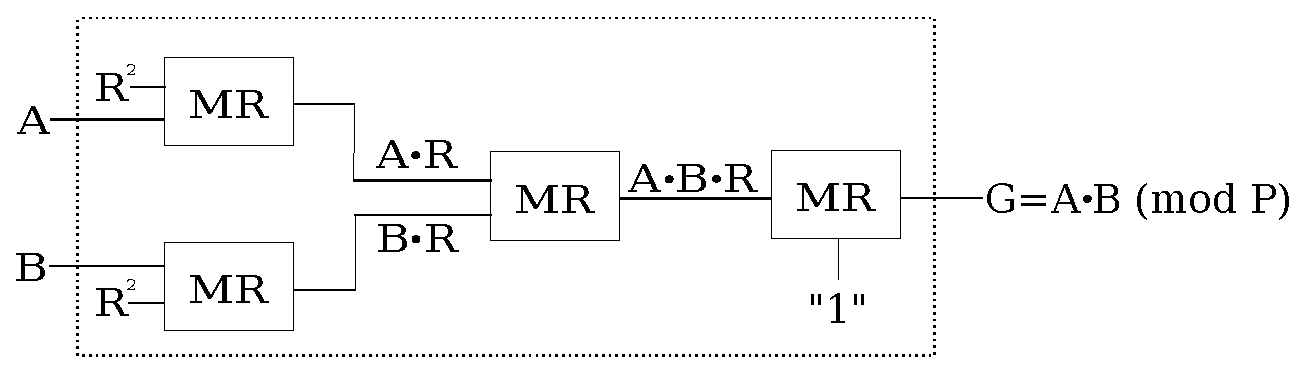
\includegraphics[scale=0.4]{new_mmcircuit.eps}
}
\caption{{\it Montgomery} multiplier over GF($2^k$)}
\label{fig:mm4}
\end{figure}
\begin{itemize}
\item Main operations in ECC rely on point additions and doubling operations
on elliptic curves over Galois fields
\item Multiplication and iterative squaring operations are usually implemented using custom-designed
Galois field multipliers
\item Given a hierarchically designed Montgomery multiplier, we will first extract polynomials AR, BR, ABR from the sub-circuit
blocks.
\item We can then apply our approach at a higher-level, to extract the function of the entire circuit.
\end{itemize}
\end{frame}
%%%%%%%%%%%%%%%%%%%%%%%%%%%%%%%%%%%%%%%%%%%%%%%%%%
\begin{frame}{\large {Galois Field Overview}}
%\vspace{-0.2in}
%\ptsize{10}
\textbf {Galois field} $\mathbb{F}_q$ is a finite field with $q$
elements, $q = p^k$
\begin{itemize}
\item Commutative Ring with unity, associate, distributive laws
\item Closure property: $+,-,\times$, inverse ($\div$)
\end{itemize}

\begin{itemize}
\item $\mathbb{F}_p \equiv (\mathbb{Z} ~\pmod{ p })$, where $p = $ prime, is a field
\begin{itemize}
\item $\mathbb{Z}_7=\{0,1,2,3,4,5,6\}$
\end{itemize}

% %\begin{comment}
% \item Ring $\mathbb{Z}_{2^k}$ ($k$-bit integer datapaths) are {\bf not} fields : 
% \begin{itemize}
% \item $\mathbb{Z}_{8}$, $\mathbb{Z}_{2^{32}}$ are not fields:
%   even numbers have no inverses
% %\item $\mathbb{R, Q, C}$ are infinite fields
% \end{itemize}
% %\end{comment}

\end{itemize}

Our interest: $\mathbb{F}_{q} = \mathbb{F}_{2^k}$, i.e. $q = 2^k$
\begin{itemize}
\item  $\mathbb{F}_{2^k}$: $k$-dimensional extension of  $\mathbb{F}_{2}$
	\begin{itemize}
	\item $k$-bit bit-vector, AND/XOR arithmetic
	\end{itemize}
\end{itemize}

To construct $\mathbb{F}_{2^k}$
\begin{itemize}
\item $\mathbb{F}_{2^k} \equiv \mathbb{F}_{2}[x] \pmod {P(x)}$
\item $P(x) \in \mathbb{F}_{2}[x]$, irreducible polynomial of degree $k$
\end{itemize}

\end{frame}
%%%%%%%%%%%%%%%%%%%%%%%%%%%%%%%%%%%%%%%%%%%%%%%%%%
%%%%%%%%%%%%%%%%%%%%%%%%%%%%%%%%%%%%%%%%%%%%%%%%%%
%\begin{comment}

\begin{frame}{\large {Field Elements: {\it e.g.} $\mathbb{F}_8$}}
%\ptsize{10}

Consider: $\mathbb{F}_{2^3}= \mathbb{F}_{2}[x] \pmod {x^3 + x +
  1}$\\ $A \in \mathbb{F}_{2}[x]$ \\ 
$A \pmod {x^3 + x + 1} = a_2 x^2 + a_1 x + a_0$. Let $P(\alpha) = 0$:

\begin{itemize}
\item $\langle a_2, a_1, a_0 \rangle = \langle 0, 0, 0\rangle = 0$
\item $\langle a_2, a_1, a_0 \rangle = \langle 0, 0, 1\rangle = 1$
\item $\langle a_2, a_1, a_0 \rangle = \langle 0, 1, 0\rangle = \alpha$
\item $\langle a_2, a_1, a_0 \rangle = \langle 0, 1, 1\rangle = \alpha
  + 1$
\item $\langle a_2, a_1, a_0 \rangle = \langle 1, 0, 0\rangle = \alpha^2$
\item $\langle a_2, a_1, a_0 \rangle = \langle 1, 0, 1\rangle =
  \alpha^2 + 1$
\item $\langle a_2, a_1, a_0 \rangle = \langle 1, 1, 0\rangle =
  \alpha^2 + \alpha$
\item $\langle a_2, a_1, a_0 \rangle = \langle 1, 1, 1\rangle =
  \alpha^2 + \alpha + 1$
\end{itemize}


\end{frame}

%\end{comment}

%%%%%%%%%%%%%%%%%%%%%%%%%%%%%%%%%%%%%%%%%%%%%%%%%%

%\begin{frame}{{Elliptic Curves -- Point addition}}

%%\ptsize{11}

%\begin{center}
%$y^2 + xy = x^3 + ax^2 + b$ over GF($2^k$)
%\end{center}

%\begin{columns}

%\begin{column}{0.3\textwidth}
%\begin{center}
%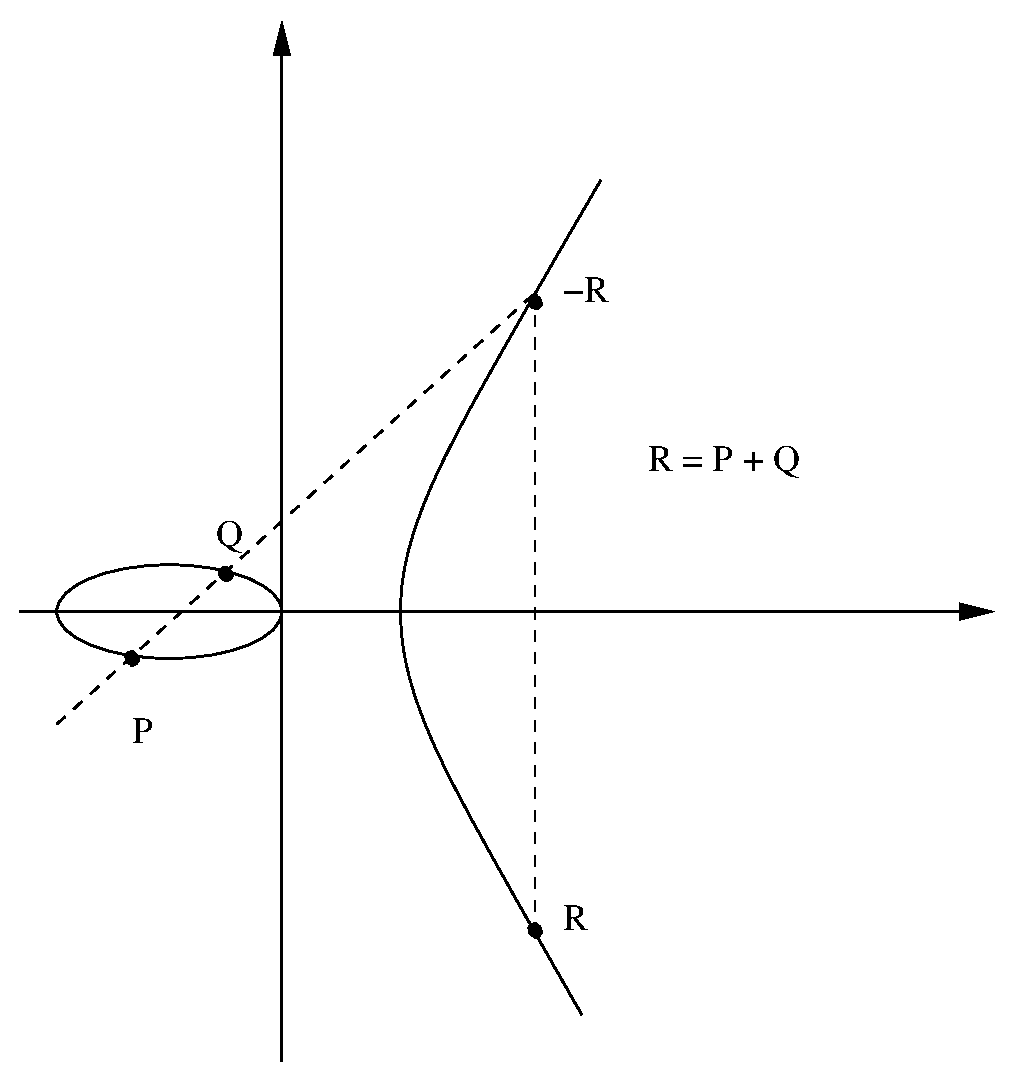
\includegraphics[height=50mm]{ecc.eps}
%\end{center}
%\end{column}
%%\end{minipage} \hfill \begin{minipage}[h]{3in}

%\begin{column}{0.3\textwidth}
%$$\text{Compute Slope:} {y_2 - y_1 \over x_2 - x_1}$$
%Computation of inverses over $\Fkk$ is expensive
%%\end{minipage}
%\end{column}

%\end{columns}
%\end{frame}


%%%%%%%%%%%%%%


%%%%%%%%%%%%%%%%%%%%%%%%%%%%%%%%%%%%%%%%%%%%%%%%%%

%\begin{frame}{{Point addition using Projective Co-ordinates}}

%\begin{itemize}
%\item Curve: ~~$Y^2 + XYZ = X^3Z + aX^2Z^2 + bZ^4$ over $\mathbb{F}_{2^k}$
%\item Let ($X_3$, $Y_3$, $Z_3$) = ($X_1$, $Y_1$, $Z_1$) + ($X_2$,
%  $Y_2$, $1$)  
%\end{itemize}

%\begin{columns}
%\begin{column}{0.2\textwidth}
%\begin{align*}
%A &= Y_2 \cdot Z_1^2 + Y_1 \\
%B &= X_2 \cdot Z_1 + X_1 \\
%C &= Z_1 \cdot B \\
%D &= B^2 \cdot(C + a Z_1^2) \\
%\alert{Z_3} &= C^2 
%\end{align*}
%\end{column} 

%\begin{column}{.3\textwidth}
%\begin{align*}
%E &= A \cdot C  \\
%\alert{X_3} &= A^2 + D + E  \\
%F &= X_3 + X_2 \cdot Z_3 \\
%G &= X_3 + Y_2\cdot Z_3 \\
%\alert{Y_3} &= E\cdot F + Z_3 \cdot G
%\end{align*}
%\end{column}
%\end{columns}

%\ \\
%No inverses, just addition and multiplication

%\end{frame}


%%%%%%%%%%%%%%


%%%%%%%%%%%%%%%%%%%%%%%%%%%%%%%%%%%%%%%%%%%%%%%%%%
\begin{frame}{\large {Multiplication in GF($2^4$)}}
%\ptsize{10}
Input: \\
$A=(a_3a_2a_1a_0)$ \\
$B=(b_3b_2b_1b_0)$ \\
$A=a_0+a_1\cdot \alpha+a_2\cdot \alpha^2+a_3\cdot \alpha^3$\\
$B=b_0+b_1\cdot \alpha+b_2\cdot \alpha^2+b_3\cdot \alpha^3$
\bigskip

Irreducible Polynomial: \\
$P=(11001)$ \\
$P(x)=x^4+x^3+1, ~~ P(\alpha) = 0$
\bigskip

Result: 

$A\times B \pmod{ P(x) }$


\end{frame}

%%%%%%%%%%%%%%%%%%%%%%%%%%%%%%%%%%%%%%%%%%%%%%%%%%
%%%%%%%%%%%%%%%%%%%%%%%%%%%%%%%%%%%%%%%%%%%%%%%%%%
\begin{frame}{\large {Multiplication over GF($2^4$)}}

 {\begin{tabular}{c c c c c c c c}
  &   &   & $a_3$ & $a_2$ & $a_1$ & $a_0$  \\ 
 $\times$&   &   & $b_3$ & $b_2$ & $b_1$ & $b_0$  \\ 
 \hline
 &   &   & $a_3\cdot b_0$ & $a_2 \cdot b_0$ & $a_1\cdot b_0$ & $a_0\cdot b_0$ \\
 &  & $a_3\cdot b_1$ & $a_2\cdot b_1$ & $a_1 \cdot b_1$ & $a_0\cdot b_1$ &   \\
 & $a_3\cdot b_2$ & $a_2\cdot b_2$ & $a_1\cdot b_2$ & $a_0\cdot b_2$ &  &   \\
 $a_3\cdot b_3$ & $a_2\cdot b_3$ & $a_1\cdot b_3$ & $a_0\cdot b_3$ &  &  &   \\
 \hline
 $s_6$& $s_5$  & $s_4$  & $s_3$ & $s_2$  & $s_1$   & $s_0$ 
 \end{tabular}\par}

\ \\
\ \\
In polynomial expression:\\
$S=s_0+s_1\cdot \alpha+s_2\cdot \alpha^2+s_3\cdot \alpha^3+s_4\cdot \alpha^4+s_5\cdot \alpha^5+s_6\cdot \alpha^6$

\bigskip

$S$ should be further reduced $\pmod {P(x)}$
\end{frame}

%%%%%%%%%%%%%%%%%%%%%%%%%%%%%%%%%%%%%%%%%%%%%%%%%%
%%%%%%%%%%%%%%%%%%%%%%%%%%%%%%%%%%%%%%%%%%%%%%%%%%
\begin{frame}{\large {Multiplication over GF($2^4$)}}

 {\begin{tabular}{c c c| c c c c |c c c}
  $s_6$& $s_5$  & $s_4$  & $s_3$ & $s_2$  & $s_1$   & $s_0$ & &  \\
 \hline
 & & &$s_4$ & $0$&$0$ &$s_4$  &$\Leftarrow$ & $s_4\cdot \alpha^4 \pmod{ P(\alpha)}$\\
 & & &$s_5$ & $0$&$s_5$ &$s_5$ & $\Leftarrow$ & $s_5\cdot \alpha^5 \pmod{ P(\alpha)}$\\
 & &$+$ &$s_6$ & $s_6$&$s_6$ &$s_6$  & $\Leftarrow$ & $s_6\cdot \alpha^6
 \pmod{ P(\alpha)}$\\
 \hline
 & & & $g_3$ & $g_2$ &$g_1$ & $g_0$
 \end{tabular}\par}

\ \\

$s_4\cdot \alpha^4 \pmod {\alpha^3+\alpha+1}=s_4\cdot \alpha^3+s_4$ \\
$s_5\cdot \alpha^5 \pmod {\alpha^3+\alpha+1}=s_5\cdot \alpha^3+s_5\cdot \alpha+s_5$ \\
$s_6\cdot \alpha^6 \pmod {\alpha^3+\alpha+1}=s_6\cdot \alpha^3+s_6\cdot \alpha^2+s_6\cdot \alpha+s_6$ 
\bigskip

$G=g_0+g_1\cdot \alpha+g_2\cdot \alpha^2+g_3\cdot \alpha^3$
\end{frame}

%%%%%%%%%%%%%%%%%%%%%%%%%%%%%%%%%%%%%%%%%%%%%%%%%%
%%%%%%%%%%%%%%%%%%%%%%%%%%%%%%%%%%%%%%%%%%%%%%%%%%

% \begin{frame}{\large {Other GF-Multiply Architectures}}

% %\ptsize{11}
% \begin{itemize}
% \item Montgomery Multipliers used for exponentiation
% \item $F = MM(A, B) = A \times B \times R^{-1} \pmod{ P(x)}$
% \item Overkill for computing $A\times B$, but much faster for
%   computing $A^{n}$.
% \end{itemize}

% \begin{center}
% \includegraphics[height=30mm]{../VLSID2011/mmcircuit.eps}
% \end{center}

% \end{frame}


%%%%%%%%%%%%%%



%%%%%%%%%%%%%%%%%%%%%%%%%%%%%%%%%%%%%%%%%%%%%%%%%%
%\begin{frame}{\large {Montgomery Architecture}}
%%\vspace{-0.2in}
%\begin{figure}[hbt]
%\centerline{
%\includegraphics[scale=0.75]{mmcircuit.eps}
%}
%\caption{{\it Montgomery} multiplier over GF($2^k$)}
%\label{fig:mm4}
%\end{figure}

%{{\it  Montgomery} Multiply: $F = A\cdot B \cdot R^{-1}$, $R = \alpha^k$}


%\begin{itemize}
%\item Barrett architectures do not require precomputed $R^{-1}$
%\item We can verify $163$-bit circuits, and also catch bugs!
%\item Conventional techniques fail beyond $16$-bit circuits
%\end{itemize}


%\end{frame}

%%%%%%%%%%%%%%%%%%%%%%%%%%%%%%%%%%%%%%%%%%%%%%%%%%

%%%%%%%%%%%%%%%%%%%%%%%%%%%%%%%%%%%%%%%%%%%%%%%%%%
\begin{frame}{\large {A Mathematical Problem}}
% \vspace{-0.2in}
% %\ptsize{10}

\begin{itemize}
\item Given \alert{circuit implementation} $C$ of a function $f: Y = \F(A)$ over $\Fkk$ and given $P(x)$, s.t. $P(\alpha) = 0$.
 \begin{itemize}
 \item Primary Input: $A = \{a_0, \dots, a_{k-1}\}$
 	\begin{itemize}
 	\item Note: we allow multiple primary inputs.
	\item i.e. $f: Y = \F(A,B,\dots)$
        \end{itemize}
 \item Primary Output $Z = \{z_0, \dots, z_{k-1}\}$
 \item $A = a_0 + a_1 \alpha + a_2\alpha^2 + \dots + a_{k-1} \alpha^{k-1}$
 \item $Z = z_0 + z_1 \alpha + \dots + z_{k-1} \alpha^{k-1}$
 \end{itemize}
\item What is the specification $Y = \F(A)$ of $C$?
\end{itemize}

Mathematically:
\begin{itemize}
\item Model the circuit (gates) as polynomials $\{f_1, \dots, f_s\}
  \in \mathbb{F}_{2^k}[x_1, \dots, x_d]$
\item Polynomial specification becomes $Y + \F(A)$
\item $Y + \F(A)$ \alert{vanishes} on the \alert{variety} of $V(f_1, \dots, f_s)$
%\item Do solutions to $f = 0$ (\alert{spec}) agree with solutions to
%  $f_1 = f_2 = \dots = f_s = 0$ (\alert{implement})?
%\item Does $f$ \alert{vanish} on the \alert{Variety} $V(f_1, \dots, f_s)$?
\end{itemize}
% \begin{itemize}
% \item If solutions exists: BUG! Otherwise, equivalence is proven
% \item SAT/SMT solvers: Search for a solution, solve systems of equations
% \item In Cryptography, $GF(2^k), k = 256$ or more
% \item SAT/SMT is infeasible. Can only solve at most $k = 16$.
% \end{itemize}

% \end{itemize}
% Our Approach: Use symbolic computer algebra and algebraic geometry to
% reason whether a given system of polynomials has a solution or not? 

\end{frame}

%%%%%%%%%%%%%%%%%%%%%%%%%%%%%%%%%%%%%%%%%%%%%%%%%%
\begin{frame}{\large {Example Formulation}}

\begin{figure}[hbt]
\centerline{
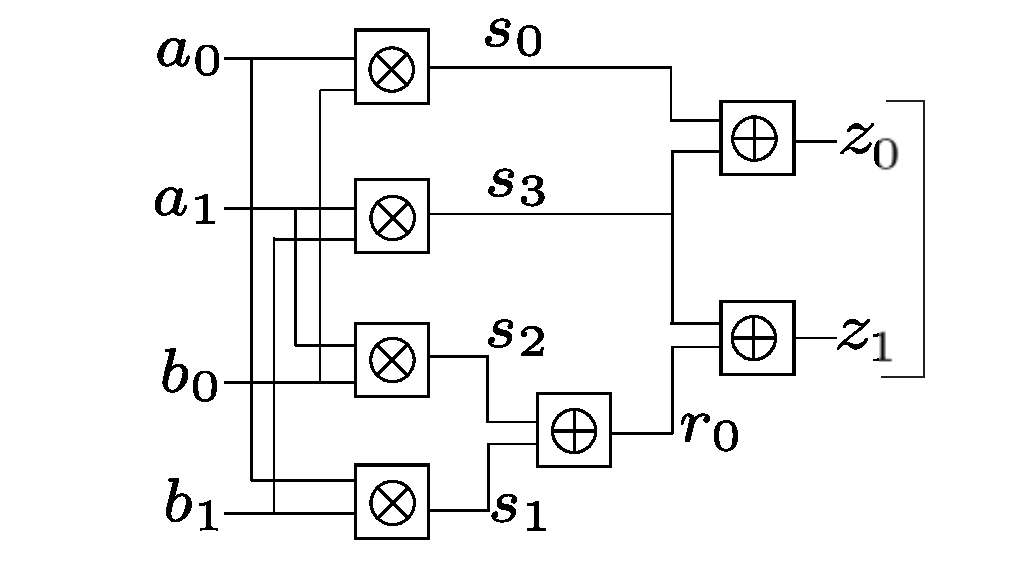
\includegraphics[scale=0.4]{2bitmult.eps}
}
%\caption{A multiplier over GF($2^2$)}
\label{fig:mult-2-bit}
\end{figure}

Model circuit as polynomials in $\mathbb{F}_2 \subset \mathbb{F}_{2^k}$:
\begin{eqnarray}
z_0 = s_0 + s_3 ~~~~ \implies ~~~~ f_1: z_0 + s_0 + s_3 \nonumber\\
s_0 = a_0\cdot b_0 ~~~~ \implies ~~~~ f_2: s_0 + a_0\cdot b_0 \nonumber\\
\vdots\nonumber\\
A + a_0 + a_1\alpha, ~~B + b_0 + b_1\alpha, ~~Z + z_0 + z_1\alpha \nonumber
\end{eqnarray}
\end{frame}
%%%%%%%%%%%%%%%%%%%%%%%%%%%%%%%%%%%%%%%%%%%%%%%%%%

%%%%%%%%%%%%%%%%%%%%%%%%%%%%%%%%%%%%%%%%%%%%

%%%%%%%%%%%%%%%%%%%%%%%%%%%%%%%%%%%%%%%%%%%%%%%%%%
\begin{frame}{\large{Computer Algebra Terminology}}
\vspace{-0.2in}
%\ptsize{10}
Let $\mathbb{F}_q = GF(2^k)$:
\begin{itemize}
\item $\mathbb{F}_q[x_1, \ldots, x_n]$: ring of all polynomials with
  coefficients in $\mathbb{F}_q$ 
\item Given a set of polynomials:
\begin{itemize}
\item $f, f_1, f_2, \dots , f_s \in \mathbb{F}_q[x_1, \dots, x_n]$
\item Find solutions to $f_1 = f_2 = \dots = f_s = 0$
\end{itemize}
\item \alert{Variety:} Set of ALL solutions to a given system of polynomial equations: $V(f_1, \dots, f_s)$
	\begin{itemize}
	\item In $\mathbb{R}\left[x,y\right]$, $V(x^2+y^2-1)=\{all\  points\  on\ circle: x^2+y^2-1=0\}$
	\item In $\mathbb{R}[x]$, $V(x^2+1)=\emptyset$
	\item In $\mathbb{C}[x]$, $V(x^2+1)=\{(\pm i)\}$
	\end{itemize}
%\item Our Problem: Is the variety empty, i.e. is $V(f_1, \dots, f_s)
%=   \emptyset$ over $\mathbb{F}_q$? 
\item Variety depends on the \alert{ideal} generated by the polynomials.
\item Reason about the Variety by analyzing the Ideals
\end{itemize}


\end{frame}
%%%%%%%%%%%%%%%%%%%%%%%%%%%%%%%%%%%%%%%%%%%%%%%%%%
%%%%%%%%%%%%%%%%%%%%%%%%%%%%%%%%%%%%%%%%%%%%%%%%%%

\begin{frame}{\large {Ideals in Rings}}
\vspace{-0.2in}
%\ptsize{10}


% \begin{Definition}
% A subset $I \subset R = \mathbb{F}_q[x_1, \dots, x_n]$ is an \textbf {ideal} if:
% \begin{itemize}
% \item $0 \in I$
% \item If $f, g \in I$, then $f + g \in I$
% \item If $f \in I$ and $h \in R$ then $f \cdot h \in I$
% \end{itemize}
% \end{Definition}

\begin{Definition}
{\bf Ideals of Polynomials:} Let $f_1, f_2, \ldots, f_s \in
\mathbb{F}_q[x_1, \dots, x_n]$. Let 
\begin{eqnarray}
J = \langle f_1, f_2 \ldots, f_s\rangle = \{f_1 h_1 + f_2 h_2 + \dots + f_s h_s\} \nonumber 
\end{eqnarray}

$J = \langle f_1, f_2 \ldots, f_s\rangle$ is an ideal generated by
$f_1, \ldots, f_s$ and the polynomials are called the generators. 
\end{Definition}


%\begin{Definition}
%{\bf Ideal Membership:} Let $f, f_1, f_2, \ldots, f_s \in
%\mathbb{F}_q[x_1, \dots, x_n]$. Let $J = \langle f_1, f_2 \ldots,
%f_s\rangle$ be an ideal $\subset \mathbb{F}_q[x_1, \dots, x_n]$. 
\begin{Definition}
{\bf Vanishing Ideal:} For any subset $V$ of $\Fq^d$, the ideal of polynomials that
vanish on $V$, called the {\it vanishing ideal of $V$}, is defined as: 
$I(V) = \{f\in \Fq[x_1,\dots, x_d]: \forall
\mathbf{a} \in V, f(\mathbf{a}) = 0\}.$


%If $f = f_1 h_1 + f_2 h_2 + \dots + f_s h_s$, then $f \in J$. 
\end{Definition}

%If $f$ is a member of the ideal $J = \langle f_1, f_2 \ldots,
%f_s\rangle$, then $f$ agrees with solutions of $f_1 = \dots = f_s = 0$.
If a polynomial $f$ vanishes on a variety $V$, then $f \in I(V)$. 
\end{frame}

%%%%%%%%%%%%%%%%%%%

\begin{frame}{\large {Example Formulation}}

\begin{figure}[hbt]
\centerline{
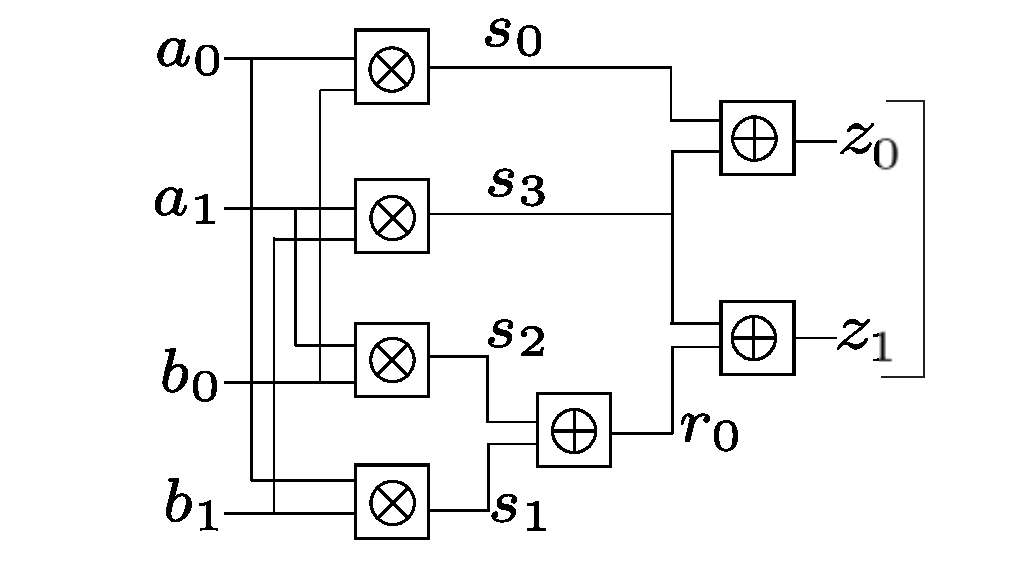
\includegraphics[scale=0.4]{2bitmult.eps}
}
%\caption{A multiplier over GF($2^2$)}
\label{fig:mult-2-bit}
\end{figure}

\begin{itemize}
\item Polynomials for all the gates: $f_1, \dots, f_s$; ideal $J =
  \langle f_1, \dots, f_s\rangle$
\item Circuit polynomial function: $f: Z = A\times B$
\item $f$ ``agrees with'' all solutions to $f_1 = \dots = f_s = 0$
\item $f$ vanishes on variety $V_{\Fkk}(J)$?
\end{itemize}

\end{frame}
%%%%%%%%%%%%%%%%%%%%%%%%%%%%%%%%%%%%%%%%%%%%%%%%%%



%%%%%%%%%%%%%%%%%%%%%%%%%%%%%%%%%%%%%%%%%%%%%%%%%%

%\begin{frame}{\large {Variety over $\mathbb{F}_q$ or over $\overline{\mathbb{F}_q}$?}}
%Where are the solutions of $f_1 = f_2 = \cdots = f_s = 0$?

%\begin{center}
%    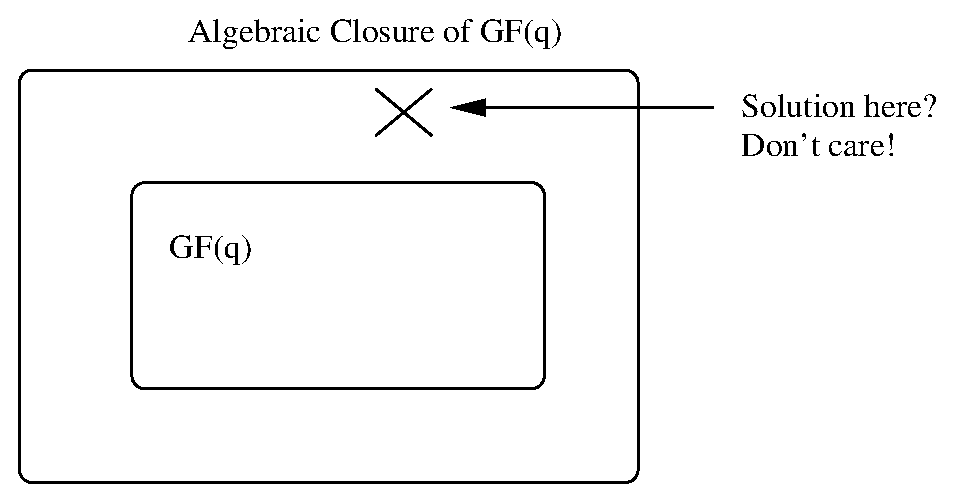
\includegraphics[scale=0.45]{gfq-closure.eps}
%\end{center}

% \begin{itemize}
% \item Property of Finite fields: $\forall x\in \mathbb{F}_q,
%   x^q-x=0$
% \item {\bf Vanishing Polynomials: $x^q - x$} are vanishing polynomials
%   of $\mathbb{F}_q$
% \item Therefore $V(x^q - x) = \mathbb{F}_q$
% \end{itemize}

%\begin{itemize}
%\item \alert{Algebraically closed field} $\mathbb{F}$: Every $f(x) \in
%  \mathbb{F}[x]$ has a root in $\mathbb{F}$
%\item Galois fields are not algebraically closed!
%\item $\overline{\mathbb{F}_q}$ = algebraic closure of $\mathbb{F}_q$:
%  $\overline{\mathbb{F}_q} \supset \mathbb{F}_q$

%\begin{itemize}
%\item Similar to $\mathbb{C} \supset \mathbb{R}$
%\end{itemize}

%\end{itemize}

%\end{frame}
%%%%%%%%%%%%%%%%%%%%%%%%%%%%%%%%%%%%%%%%%%%%%%%%%%

%\begin{frame}{\large {Restricting the Variety to $\mathbb{F}_q$?}}

%\begin{center}
%    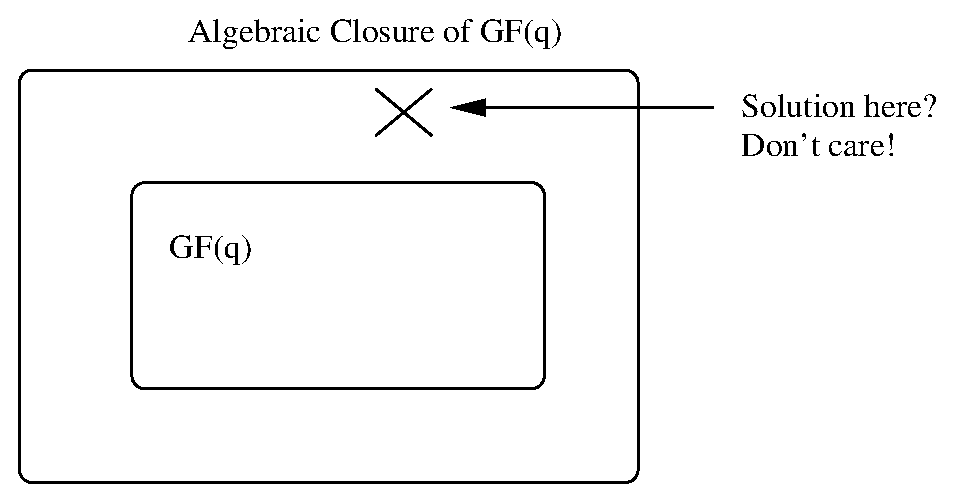
\includegraphics[scale=0.45]{gfq-closure.eps}
%\end{center}

% \begin{itemize}
% \item Property of Finite fields: $\forall x\in \mathbb{F}_q, x^q-x=0$
% \item {\bf Vanishing Polynomials: $x^q - x$} are vanishing polynomials
%   of $\mathbb{F}_q$
% \item Therefore $V(x^q - x) = \mathbb{F}_q$
% \item Restrict the solutions to $\mathbb{F}_q$: $V_{\mathbb{F}_q}(f_1, \dots, f_s) =
%   V_{\overline{\mathbb{F}_q}}(f_1, \dots, f_s, ~~x_1^q - x_1, \dots,  x_n^q - x_n)$
% \end{itemize}


%\end{frame}



%%%%%%%%%%%%%%%%%%%%%%%%%%%%%%%%%%%%%%%%%%%%%%%%%%

\begin{frame}{\large {Strong Nullstellensatz over $\Fq$} }
\begin{Definition}
{\bf Vanishing Polynomials:}
Polynomials of the form $\{x^q - x\}$ over $\Fq$. Let $F_0 = \{x_1^q - x_1,
\dots, ~x_d^q - x_d\}$, then $J_0 = \langle x_1^q - x_1, \dots, x_d^q
- x_d\rangle$ is the ideal of all vanishing polynomials in
$\mathbb{F}_q[x_1,\dots,   x_d]$.
\end{Definition}
\begin{itemize}
\item For any Galois field $\Fq$, let $J \subseteq \Fq[x_1,\dots,x_d]$ be an ideal, and let 
$J_0 = \langle x_1^q - x_1, \dots, x_d^q - x_d\rangle$ be
the ideal of all vanishing polynomials.
\item Let $V_{\Fq}(J)$ denote the
variety of $J$ over $\Fq$.
\item Then, $I(V_{\Fq}(J)) = J + J_0 = J +
\langle  x_1^q - x_1, \dots, ~x_d^q - x_d\rangle$.
\end{itemize}
\end{frame}

%%%%%%%%%%%%%%%%%%%%%%%%%%%%%%%%%%%%%%%%%%%%%%%%%%%%
\begin{frame}{\large {Our Problem Formulation}}
Given circuit $C$ which implements a polynomial function $Y = \F(A)$ over
  $\mathbb{F}_q[x_1, \dots, x_n]$
\begin{itemize}
\item $Y + \F(A)$ is the polynomial specification of $C$
\item $J = \langle f_1, f_2 \ldots, f_s\rangle$, Polynomials from the design
\item $J_0 = \langle x_1^q  - x_1, \dots, x_n^q - x_n\rangle$,
  Vanishing polynomials generated
\item $J + J_0 = \langle f_1, f_2 \ldots, f_s, ~~ x_1^q
  - x_1, \dots, x_n^q - x_n\rangle$;  Variety $V(J + J_0) = $ circuit configuration
\item $Y + \F(A) \in J + J_0$
\end{itemize}

\ \\
% Recall: If $f = f_1 h_1 + f_2 h_2 + \dots + f_s h_s$, then $f
%   \in \langle f_1, \dots, f_s\rangle$
% \begin{itemize}
% \item To test if $f \in \langle f_1, \dots, f_s\rangle$? Intuitively,
% \item Divide $f \stackrel{f_1, f_2, \cdots,
%     f_s}{\textstyle\longrightarrow}_+r$. If $r = 0 \implies f
%   \in \langle f_1, \dots, f_s\rangle$.
% \item But what if $r\neq 0$? $f$ may still be in the ideal!

% \end{itemize}

% Need a complete decision procedure....

%Since $f$ vanishes on $V_{\Fq} (J)$, then:\\
\begin{center}
% $f \in I(V_{\Fq}(J)) = I(V_{\overline{\Fq}}(J + J_0)) = \sqrt{J +
%   J_0} = J + J_0$\\
%\ \\
Our problem: Find the polynomial specification $Y + \F(A) \in (J + J_0)$\\

Requires the computation of a \alert{Gr\"obner basis of $J + J_0$}
\end{center}
\end{frame}

%%%%%%%%%%%%%%%%%%%%%%%%%%%%%%%%%%%%%%%%%%%%%%%%%%
\begin{frame}{\large {Specification Abstraction Requires a Gr\"obner Basis}}
\vspace{-0.2in}
%\ptsize{10}

\begin{itemize}
\item Different generators can generate the same ideal
\item $\langle f_1,\cdots,f_s \rangle=\cdots=\langle g_1,\cdots,g_t
  \rangle$
\item Some generators are a ``better'' representation of the ideal
\item A {\bf Gr\"obner basis} is a ``canonical'' representation of an ideal
\end{itemize}

Given $F = \{f_1, f_2,\cdots, f_s\}$, Compute a Gr\"obner Basis $G =
\{g_1,g_2,\cdots,g_t\}$, such that $I = \langle F \rangle = \langle G \rangle$

\begin{center}
$V(F)=V(G)$
\end{center}

%Grobner Basis $G$ decides ideal membership:\\
%\begin{center}
%$G = GB(I) \iff \forall f \in I, f \stackrel{g_1, g_2, \cdots,
%  g_t}{\textstyle\longrightarrow}_+0$ 
%\end{center}

\end{frame}

%%%%%%%%%%%%%%%%%%%%%%%%%%%%%%%%%%%%%%%%%%%%%%%%%%

\begin{frame}{\large{Buchberger's Algorithm Computes a Gr\"obner Basis}}

%{\small
%\begin{algorithm}
%\caption {Buchberger's Algorithm}
{\bf Buchberger's Algorithm}\\
%\label{alg:gb}
%\begin{algorithmic}
% \REQUIRE : $F = \{f_1, \dots, f_s\}$
 INPUT : $F = \{f_1, \dots, f_s\}$\\
% \ENSURE : $G = \{g_1,\dots ,g_t\}$\\ %, a Gr\"{o}bner basis \\
 OUTPUT : $G = \{g_1,\dots ,g_t\}$\\ %, a Gr\"{o}bner basis \\
  $G:= F$; \\
  REPEAT\\
  \hspace{0.1in} $G' := G$\\
  \hspace{0.1in} For each pair $\{f, g\}, f \neq g$ in $G'$ DO\\
\hspace{0.2in}  $S(f, g) \stackrel{G'}{\textstyle\longrightarrow}_+
r$ \\
\hspace{0.2in}  IF $r \neq 0$ THEN $G:= G \cup \{r\}$ \\
%\hspace{0.2in}  $G(x):=G(x) / x$
UNTIL $G = G'$
%\end{algorithmic}
%\end{algorithm}

\[
S(f,g)=\frac{L}{lt(f)}\cdot f - \frac{L}{lt(g)}\cdot g
\]
$L = \text{LCM}(lm(f), lm(g))$, ~~$lm(f)$: leading monomial of $f$
%}

\end{frame}

%%%%%%%%%%%%%%%%%%%%%%%%%%%%%%%%%%%%%%%%%%%%%%%%%%

\begin{frame}{\large {Complexity of Gr\"obner Basis and Term Orderings}}
%\ptsize{10}
\begin{itemize}
\item For $J \subset \mathbb{F}_q[x_1, \dots, x_n]$, Complexity
  $GB(J + J_0): q^{O(n)}$
\item GB complexity very sensitive to {\bf term ordering}
\item A term order has to be imposed for systematic polynomial computation
\end{itemize}

Let $f = 2x^2yz + 3xy^3 - 2x^3$
\begin{itemize}
\item LEX $x> y> z$: ~~$f = {\bf -2x^3} + 2x^2yz + 3xy^3$
\item  DEGLEX $x>y>z$:  ~~$f = {\bf 2x^2yz} + 3xy^3 -2x^3$
\item DEGREVLEX $x>y>z$: ~~$f = {\bf 3xy^3} + 2x^2yz - 2x^3$
\end{itemize}
Recall, S-polynomial depends on term ordering:
\[
S(f,g)=\frac{L}{lt(f)}\cdot f - \frac{L}{lt(g)}\cdot g;
~~~~~~L = \text{LCM}(lm(f), lm(g))
\]

\end{frame}

%%%%%%%%%%%%%%%%%%%%%%%%%%%%%%%%%%%%%%%%%%%%%%%%%%


\begin{frame}{\large {Elimination Theorem}}
\begin{itemize}
\item Let $J \subset \Fq[x_1,\dots,x_d]$ be an ideal
\end{itemize}
\begin{itemize}
\item Let $G$ be a \Grobner basis of $J$ with respect to a lex ordering where $x_1
> x_2 > \dots > x_d$.
\end{itemize}
\begin{itemize}
\item Then for every $0 \leq l \leq d$:
	\begin{itemize}	
	\item The set $G_l= G \cap \Fq[x_{l+1},\dots,x_d]$ is a Gr\"obner basis of the $l$th elimination ideal $J_l$.
	\end{itemize}
\end{itemize}

The $l$th elimination ideal does not contain variables
$x_1,\dots,x_l$, nor do the generators of it.

\end{frame}

%%%%%%%%%%%%%%%%%%%%%%%%%%%%%%%%%%%%%%%%%%%%%%%%%%

\begin{frame}{\large {Elimination Term Ordering Example}}
%\ptsize{10}
\begin{itemize}
\item Let ideal $I = \langle f_1, f_2, f_3 \rangle$ where
	\begin{itemize}
	\item $f_1 = x^2 + y + z - 1$
	\item $f_2 = x + y^2 + z - 1$
	\item $f_3 = x + y + z^2 - 1$
	\end{itemize}
\item The \Grobner basis of $I$ with lex order $(x > y > z)$ is
	\begin{itemize}
	\item $g_1 = x + y + z^2 - 1$
	\item $g_2 = y^2 - y - z^2 + z$
	\item $g_3 = 2yz^2 + z^4 - z^2$
	\item $g_4 = z^6 - 4z^4 + 4z^3 - z^2$
	\end{itemize}
\item Notice that $g_2$ and $g_3$ only contain variables $y$ and $z$
	\begin{itemize}
	\item Eliminates variable $x$
	\end{itemize}
\item Similarly, $g_4$ only contains the variable $z$ and eliminates $x$ and $y$
\end{itemize}
\end{frame}

%%%%%%%%%%%%%%%%%%%%%%%%%%%%%%%%%%%%%%%%%%%%%%%%%%

\begin{frame}{\large {Abstraction Term Ordering}}

Derived from applying elimination theorem to our problem set
\begin{itemize}
\item Given a circuit $C$ implementing $Y = \F(A)$ over $\Fq$
\item Using the variable order $x_1 > x_2 > \dots > x_d > Y > A$
	\begin{itemize}
	\item $x_1, \dots ,x_d$ are the circuit polynomials
	\end{itemize}
\item Impose a lex term order $>$ on the polynomial ring $R = \Fq[x_1,
  \dots, x_d, Y, A]$.
\item This elimination term order $>$ is defined as
the {\bf Abstraction Term Order}.

\item If we compute a Gr\"obner basis $G$ of ideal $(J
+ J_0)$ using the abstraction term order $>$
	\begin{itemize}
	\item $G$ will contain the vanishing polynomial $A^q - A$ as the only
	polynomial with only $A$ as the support variable
	\item $G$ will contain a polynomial of the form $Y + \F(A)$
	\item $Y + \F(A)$ is a \alert{unique, canonical, polynomial}
  representation of $C$ over $\Fq$ 
%	\item $Y + {\mathcal{G}}(A)$ is such that $\F(A) = {\mathcal{G}}(A),
%	\forall A \in \Fq$.
%		\begin{itemize}
%		\item In other words, ${\mathcal{G}}(A)$ and $\F(A)$ are
%equal polynomial functions over $\Fq$.
%		\item  is a \alert{unique, canonical, polynomial}
%  representation of the circuit
%		\end{itemize}
	\end{itemize}
\end{itemize}
\end{frame}

%%%%%%%%%%%%%%%%%%
%\begin{frame}{\large Effect of Term Orderings}

%If $lm(f) \cdot lm(g) = LCM(lm(f), lm(g))$, 
%then $S(f,g)\stackrel{G'}{\textstyle\longrightarrow}_+ 0.$\\
%\ \\
%{\small
%LEX: $x_0 > x_1 > x_2 > x_3$
%\begin{itemize}
%\item $f=x_0 x_1+x_2$, $g=x_1x_2+x_3$
%\item $lm(f) = x_0 x_1; ~~ lm(g) = x_1 x_2$
%\item $S(f, g) \stackrel{G'}{\textstyle\longrightarrow}_+ x_0x_3 + x_2^2$
%\end{itemize}
%
%LEX: $x_3 > x_2 > x_1 > x_0$
%\begin{itemize}
%\item $f=x_2 + x_0 x_1$, $g=x_3 + x_1x_2$
%\item $lm(f) = x_2; ~~ lm(g) = x_3$, $S(f, g) \stackrel{G'}{\textstyle\longrightarrow}_+ 0$
%\end{itemize}
%}

%Problem: Find a ``term order'' that makes ALL $\{lm(f), ~lm(g)\}$ 
%relatively prime.

%\end{frame}

%%%%%%%%%%%%%%%%%%%%%%%%%%%%%%%

\begin{frame}{\large{Abstraction Term Order Example}}

\centerline{
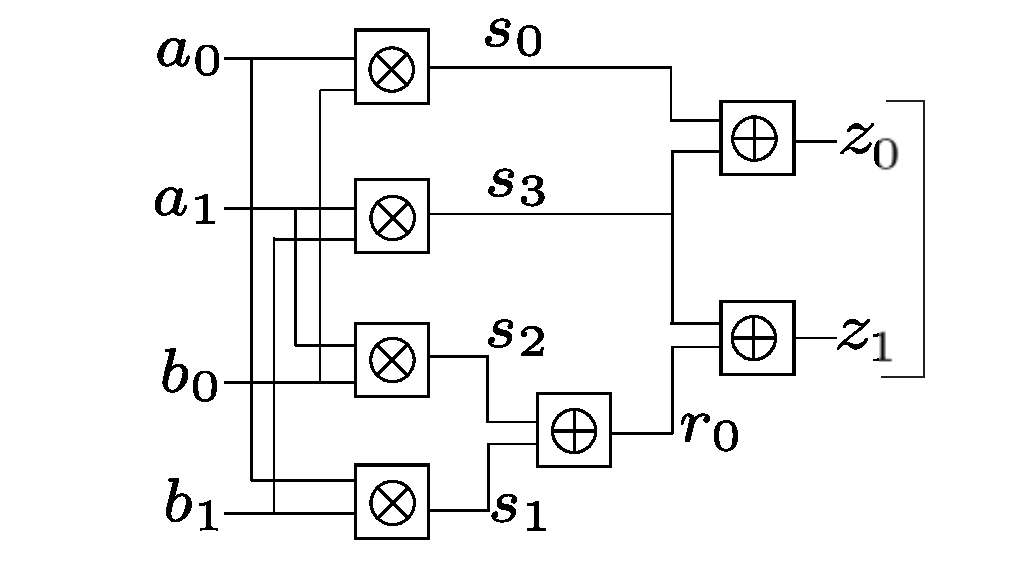
\includegraphics[scale=0.4]{2bitmult.eps}
}
%\vspace{-0.3in}
{\bf $(z_0 > z_1 > r_0 > s_0 > s_3 > s_1 > s_2 > a_0 > a_1 >  b_0 > b_1 > Z > A > B)$}
\begin{align*}
f_1: s_0+a_0 \cdot b_0; ~~f_2: s_1+a_0 \cdot b_1;  ~~f_3: s_2+a_1 \cdot b_0; ~~f_4: s_3+a_1 \cdot b_1  \nonumber \\
f_5: r_0+s_1 + s_2; ~~f_6: z_0+s_0 + s_3; ~~f_7: z_1+r_0+s_3; ~~f_8: a_0 + a_1 \alpha + A \nonumber \\ 
f_9: b_0 + b_1 \alpha + B; ~~f_{10}: z_0 + z_1 \alpha + Z \nonumber
\end{align*}
\vspace{-0.3in}
{\bf $J$ = $\langle f_1, \dots, f_{10} \rangle$}
\end{frame}

%%%%%%%%%%%%%%%%%%%%%%%%%%%%%%%

\begin{frame}{\large{Abstraction Term Order Example}}

\centerline{
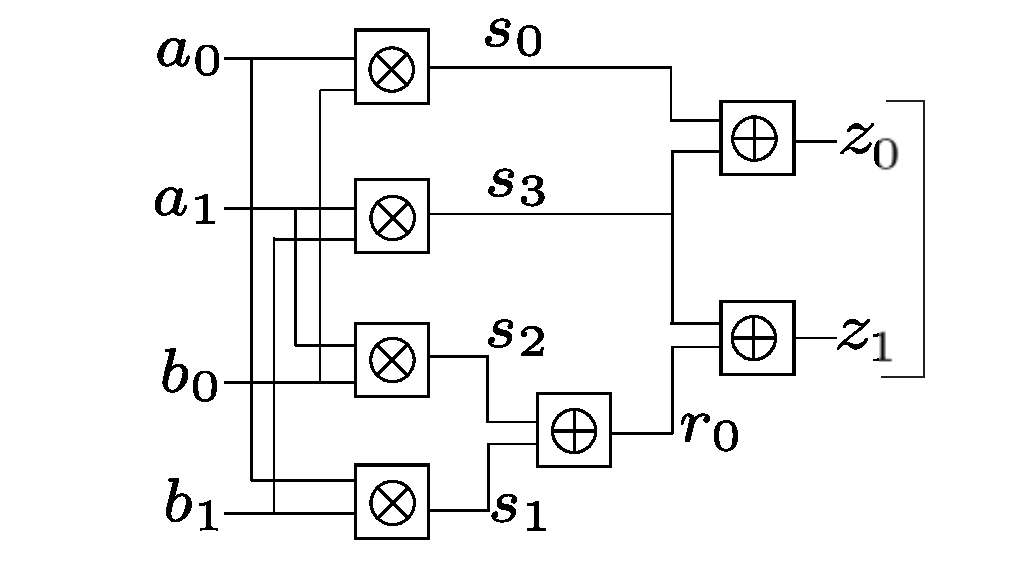
\includegraphics[scale=0.4]{2bitmult.eps}
}
%\vspace{-0.3in}
{\bf $(z_0 > z_1 > r_0 > s_0 > s_3 > s_1 > s_2 > a_0 > a_1 >  b_0 > b_1 > Z > A > B)$}
\begin{align*}
f_{11}: a_0^2+a_0; ~~f_{12}: a_1^2+a_1 \alpha; ~~f_{13}: b_0^2+b_0; ~~f_{14}: b_1^2+b_1; ~~f_{15}: s_0^2+s_0;  \nonumber \\
f_{16}: s_1^2+s_1; ~~f_{17}: s_2^2+s_2; f_{18}: s_3^2+s_3; ~~f_{19}: r_0^2+r_0; ~~f_{20}: z_0^2+z_0 \nonumber \\
f_{21}: z_1^2+z_1; ~~f_{22}: A^4+A; ~~f_{23}: B^4+B; ~~f_{24}:Z^4+Z \nonumber
\end{align*}
\vspace{-0.3in}
{\bf $J_0$ = $\langle f_{11}, \dots, f_{24} \rangle$}
\end{frame}

%%%%%%%%%%%%%%%%%%%%%%%%%%%%%%%

\begin{frame}{\large{Abstraction Term Order Example}}

\centerline{
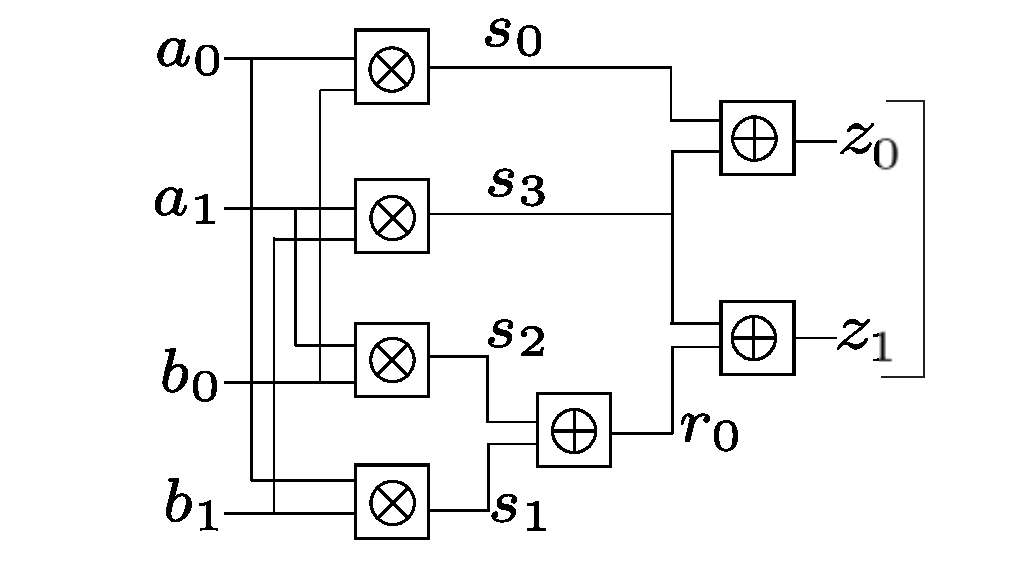
\includegraphics[scale=0.4]{2bitmult.eps}
}
%\vspace{-0.3in}
{\bf $(z_0 > z_1 > r_0 > s_0 > s_3 > s_1 > s_2 > a_0 > a_1 >  b_0 > b_1 > Z > A > B)$}

Compute the \Grobner basis, $G$, of \{$J + J_0$\} with respect to abstraction term ordering $>$.
$G$ = \{$g_1, \dots, g_{14}$\}
\begin{align*}
g_1: B^4+B; ~~g_2: b_0+b_1 \alpha + B; ~~g_3: a_0+a_1 \alpha + A; ~~g_4: A^4+A; \nonumber \\
g_5: s_0+s_1 \alpha + s_2 (\alpha + 1) + Z; ~~g_6: r_0+s_1+s_2; ~~g_7: z_1+r_0+s_3 \nonumber \\
g_7: z_0+z_1 \alpha +Z; ~~{\bf g_9: Z+A*B} ; ~~g_{10}: b_1+B^2+B; ~~g_{11}: a_1+A^2+A \nonumber \\
g_{12}: s_3+a_1 b_1; ~~g_{13}: s_2+a_1 b_1 \alpha +a_1 B; ~~g_{14}: s_1+a_1 b_1 \alpha +b_1 A  \nonumber
\end{align*}

\end{frame}

%%%%%%%%%%%%%%%%%%%%%%%%%%%%%%

\begin{frame}{\large{Complexity of \Grobner Basis over Abstraction Term Ordering}}
\begin{table}[t]
	\begin{center}
	    \caption{Runtime of Gr\"obner Basis Computation}\label{tab:sT}
	    \begin{tabular}{|c|c||c|} 
	        \hline
		{\bf Word Size ($k$)} & {\bf Number of Polynomials ($d$) } & {\bf Time (minutes) }  \\
		\hline
	        $16$	&  $1,871$  & $2.4$ \\
		\hline
		$24$	&  $3,135$  & $12$  \\
		\hline
	        $32$	&  $5,549$  & $22.6$ \\
		\hline
	        $40$	&  $8,587$  & $266$ \\
		\hline
		$48$	& $12,327$  & NA (Out of Memory) \\
	        \hline
	    \end{tabular}
	\end{center} 
\end{table}
\begin{itemize}
\item Mastrovito multiplier circuits
\item Extract Boolean gate-level operators $J$ and vanishing polynomials $J_0$
\item Compute Gr\"obner basis of $J + J_0$ with respect to our term order $>$
	\begin{itemize}
	\item Resulting Gr\"obner basis contains a polynomial $Y + A \times B$  
	\end{itemize}
\item Gr\"obner basis computed using Singular's "slimgb" command
	\begin{itemize}
	\item Run on a 64-bit Ubuntu machine with a 2.4GHz CPU and 8Gb of RAM
	\item Unable to perform Gr\"obner basis computations of multipliers beyond 40-bit word inputs
	\end{itemize}
\end{itemize}
\end{frame}

%%%%%%%%%%%%%%%%%%%%%%%%%%%%%%

\begin{frame}{\large {FGLM Algorithm}}
\vspace{-0.2in}

\begin{itemize}
\item Takes as input a \Grobner basis, $G_1$, and two monomial term orderings, $>_a$ and $>_b$.
	\begin{itemize}
	\item $G_1$ must be a \Grobner basis over term ordering $>_a$
	\end{itemize}
\end{itemize}

\begin{itemize}
\item Converts $G_1$ to a \Grobner basis over term ordering $>_b$
\end{itemize}

{\bf Applying FGLM to our approach:}
\begin{itemize}
	\item Given a circuit C which performs $Y = \F(A)$ over $\Fkk$
	\item Find the \Grobner basis, $G_1$, of \{$J+J_0$\} in a convenient term ordering
	\item Using FGLM, convert $G_1$ to a \Grobner basis, $G_2$, over abstraction term ordering $>$
	\item $G_2$ will contain a polynomial $Y + \F(A)$
\end{itemize}


\end{frame}

%%%%%%%%%%%%%%%%%%%%%%%%%%%%%%

\begin{frame}{\large{\Grobner Basis of $J + J_0$ Without Computation}}
Past contribution by Lv:

\begin{itemize}
\item Given a circuit $C$ which implements $Y = \F(A)$ over $\Fkk$
\end{itemize}
\begin{itemize}
\item Using the lex variable order $Y > A > x_1 > x_2 > \dots > x_d$
	\begin{itemize}
	\item Where $x_1 \dots x_d$ are bit-level circuit variables in \alert{reverse topographical order}
	\end{itemize}
\end{itemize}
\begin{itemize}
\item $J + J_0$ is itself a \Grobner basis
\end{itemize}

No \Grobner basis computation necessary!

We denote this term order as $>_1$
\end{frame}

%%%%%%%%%%%%%%%%%%%%%%%%%%%%%%

\begin{frame}{\large{Variable Term Order $>_1$ Example}}

\centerline{
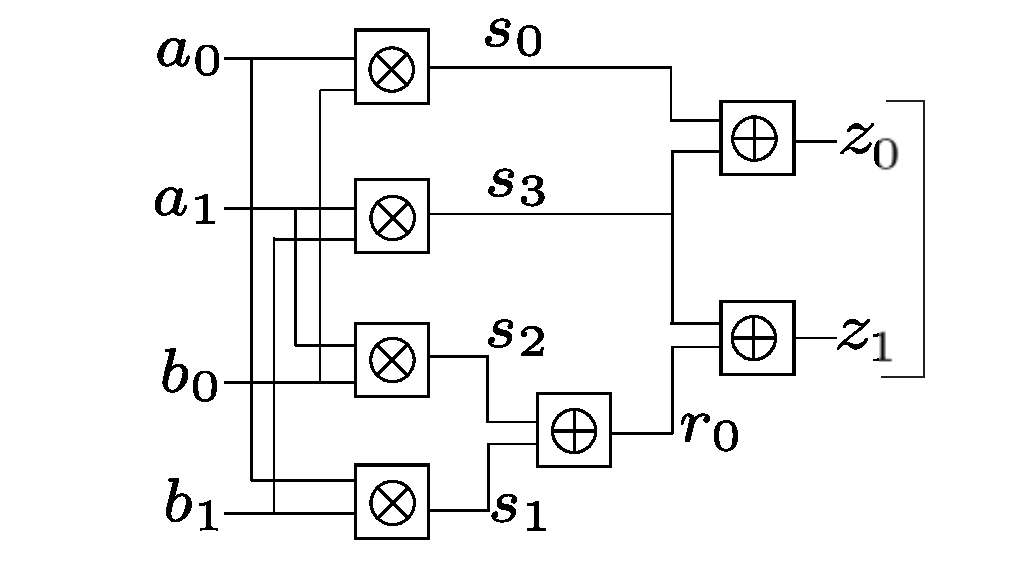
\includegraphics[scale=0.4]{2bitmult.eps}
}

{\bf $(Z > A > B > z_0 > z_1 > r_0 > s_0 > s_3 > s_1 > s_2 > a_0 > a_1 > b_0 > b_1)$}

\vspace{0.3in}
\begin{itemize}
\item Same $J$ and $J_0$ as shown previously
\item $J+J_0$ denote a \Grobner basis over term ordering $>_1$
\end{itemize}
\end{frame}

%%%%%%%%%%%%%%%%%%%%%%%%%%%%%%

\begin{frame}{\large {Proposed Approach}}
Proposed approach to extract a unique polynomial representation $Y = \F(A)$ of circuits over $F_{2^k}$
while obviating \Grobner basis calculation:
\begin{itemize}
\item Let $C$ be a circuit performs the function $f:
\B^k \rightarrow \B^k$
\item Extract the polynomials from
the circuit (ideal $J$) and vanishing polynomials (ideal $J_0$)
\item Assign the monomial ordering $>_1$; this makes $J+J_0$ a 
minimal Gr\"obner basis, $G_1$
\item Use the FGLM algorithm to transform
$G_1$ to a \Grobner basis, $G_2$, over abstraction ordering $>$
\item $G_2$ will contain a polynomial in the form of $Y + \F(A)$, 
where $Y$ is the word output and $A$ is the word input of the circuit
	\begin{itemize}	
	\item $Y + \F(A)$ is the {\bf unique polynomial representation} for $C$ over $f: \Fkk \rightarrow \Fkk$
	\end{itemize}
\end{itemize}
\end{frame}

%%%%%%%%%%%%%%%%%%%%%%%%%%%%%%

\begin{frame}{\large {FGLM Algorithm Overview}}
\begin{itemize}
\item FGLM starts by taking the least monomial in our abstraction term 
ordering, $A$.
\item Starting with $m=0$, it computes $[A^m$ mod $G_1]$
	\begin{itemize}
	\item Stores the remainder, $r$
	\end{itemize} 
\item Checks to see if the remainder is a combination of any previous remainders calculated thus far.
\item If so, it adds this 
representation to $G_2$ and moves on to the next monomial, else it 
increments $m$.
\end{itemize}

How exactly FGLM computes if $r$ is a combination of previous remainders, and how it finds this combination, is still being investigated
\end{frame}

%%%%%%%%%%%%%%%%%%%%%%%%%%%%%%

\begin{frame}{\large {FGLM Algorithm Example}}
\begin{itemize}
\item $A^0 = 1$
\item $A^1 = a_0+ a_1 \alpha$
\item $A^2 = a_0+a_1 \cdot (\alpha+1) $
\item $A^3 = a_0 \cdot a_1+a_0+a_1$
\item $A^4 = a_0+ a_1 \alpha = A$
\end{itemize}

$A^4$ can be composed of $A$, so $A + A^4$ is added to \Grobner basis 

\begin{itemize}
\item $B^1 = b_0+(\alpha) \cdot b_1$
\item $B^2 = b_0+(\alpha+1) \cdot b_1$
\item $B^3 = b_0 \cdot b_1+b_0+b_1$
\item $B^4 = b_0+(\alpha) \cdot b_1 = B$
\end{itemize}

$B^4$ can be composed of $B$, so $B + B^4$ is added to \Grobner basis

\begin{itemize}
\item $Z^1 = a_0 \cdot b_0 + a_0 \cdot b_1 \cdot \alpha + a_1 \cdot b_0 \cdot \alpha + a_1 \cdot b_1 \cdot \alpha^2 \linebreak
= (a_0 + a_1 \cdot \alpha) \cdot (b_0 + b_1 \cdot \alpha) = A \cdot B$
\end{itemize}

$Z + A \cdot B$ is added to \Grobner basis

\end{frame}

%%%%%%%%%%%%%%%%%%%%%%%%%%%%%%

\begin{frame}{\large {FGLM-Related Research}}
\begin{itemize}
\item FGLM continues to convert every monomial to the new term order
\item However, we only care about the word-level variables found in the $Y + \F(A)$ polynomial
\item We can make the FGLM more efficient for our approach by restricting it to only compute the word-level variables
\item Singular contains an FGLM implementation ('fglm' command)
	\begin{itemize}
	\item Propose to modify Singular's implementation
	\end{itemize}
\end{itemize}
\end{frame}

%%%%%%%%%%%%%%%%%%%%%%%%%%%%%%%

\begin{frame}{\large {Proposed Contributions}}
\begin{itemize}
\item Explore the implementation of Singular's FGLM algorithm.
\item Develop an efficient CAD tool FGLM implementation which only performs ordering conversions on the required monomials. 
\item Research the complexity and feasibility of our given approach over large circuits.
\item Apply the approach to elliptic curve cryptography circuits - particularly hierarchically designed multipliers and point addition circuits.
\end{itemize}
\end{frame}

%%%%%%%%%%%%%%%%%%%%%%%%%%%%%%%

\begin{frame}{\large {Proposed Timeline}}
\begin{itemize}
\item Spring 2013: Research FGLM algorithm in more detail. Study and analyze the source code of Singular's FGLM implementation.
\item Early Summer 2013: Develop modified FGLM implementation. Run experiments on circuits of various sizes using proposed approach with the modified FGLM algorithm.
\item Late Summer 2013: Evaluate data. Write Thesis.
\end{itemize}
\end{frame}

\begin{comment}
\begin{frame}{Questions?}
\bigskip
\vspace{0.9in}
\hspace{1.5in}
Vielen Dank! \\
\bigskip
\hspace{1.5in}
Questions?
\end{frame}
\end{comment}
%%%%%%%%%%%%%%%%%%%%%%%%%%%%%%


% \end{document}
\begin{frame}{\large OLD STUFF}
\end{frame}

%%%%%%%%%%%%%%%%%%%%%%%%%%%%%%%%%
\begin{frame}{\large{Our Discovery: Gr\"obner Basis of $J + J_0$}}

Using Our Topological Term Order:
\begin{itemize}
\item $F = \{ f_1, \dots, f_s\}$ is a Gr\"obner Basis of $J = \langle
  f_1, \dots, f_s\rangle$
\item $F_0 = \{x_1^q - x_1, \dots, x_n^q - x_n\}$ is also a Gr\"obner
  basis of $J_0$
\item But we have to compute a Gr\"obner Basis of $J + J_0 = \langle
  f_1, f_2 \ldots, f_s, ~~ x_1^q   - x_1, \dots, x_n^q - x_n\rangle$
\item We show that $\{f_1, f_2 \ldots, f_s, ~~ x_1^q   - x_1, \dots,
  x_n^q - x_n\}$ is a Gr\"obner basis!!
\item From our circuit: $f_i = x_i + P$
\item Only pairs to consider: $S(f_i, ~~~x_i^q - x_i)$ in Buchberger's Algorithm:
\end{itemize}

\[
S(f_i, ~~~x_i^q - x_i) \stackrel{J}{\textstyle\longrightarrow}_+ P^q -
P \stackrel{J_0}{\textstyle\longrightarrow}_+ 0
\]

Conclusion: Our term order makes $\{f_1, \dots, f_s, x_1^q - x_1,
\dots, x_n^q - x_n\}$ a Gr\"obner Basis
\end{frame}

%%%%%%%%%%%%%%%%%%%%%%%%%%%%%%%%%
\begin{frame}{\large Lv's Term Order: Already a Gr\"obner basis}

\centerline{
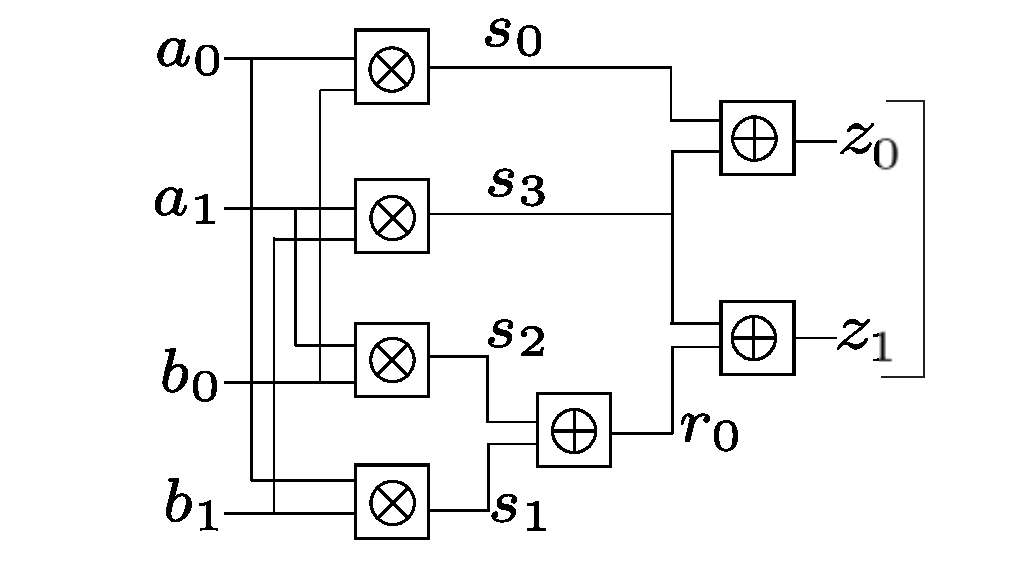
\includegraphics[scale=0.4]{2bitmult.eps}
}
\vspace{-0.3in}
\begin{align*}
f_1: s_0+a_0 \cdot b_0, \ lm=s_0; ~~~s_0^q - s_0 \nonumber \\
f_2: s_2+a_1 \cdot b_0, \ lm=s_2; ~~~s_2^2 - s_2 \nonumber \\
\end{align*}
\vspace{-0.5in}

\begin{itemize}
\item Every gate: $f_i: x_i + P \in J$
\item Every vanishing polynomial: $x_i^q - x_i \in J_0$
\end{itemize}
$S(f_i, ~~~x_i^q - x_i) \stackrel{J}{\textstyle\longrightarrow}_+ P^q -
P \stackrel{J_0}{\textstyle\longrightarrow}_+ 0
$

$\{f_1, \dots, f_s, ~~x_1^q - x_1, \dots, x_n^q - x_n \}$  is a
Gr\"obner basis
\end{frame}



%%%%%%%%%%%%%%%%%%%%%%%%%%%%%%%%%%%%%%%%%%%%%%%%%%

\begin{frame}{Our  Overall Approach}

\begin{itemize}
\item Given the circuit, perform reverse topological traversal
\item Derive the term order to represent the polynomials for every gate
\item The set: $\{F, F_0\} = \{f_1, \dots, f_s, ~~x_1^q - x_1, \dots, x_n^q -
  x_n\}$ is a Gr\"obner Basis
\item Obtain: $f \stackrel{F, F_0}{\textstyle\longrightarrow}_+ r$
\item If $r = 0$, the circuit is correct
\item If $r \neq 0$, then $r$ contains only the \alert{primary input
    variables}
\item Any SAT assignment to $r\neq 0$ generates a counter-example
\item Counter-example found in no time as $r$ is simplified by Gr\"obner basis reduction
\end{itemize}

\end{frame}


%%%%%%%%%%%%%%%%%%%%%%%%%%%%%%%%%%%%%%%%%%%%%%%%%%

%\begin{frame}{\large{Experimental Results: Correctness Proof}}
%\vspace{-0.2in}
%%\ptsize{8}

%{\small
%\begin{table}[h!]
%\begin{center}
%\caption{Verification Results of SAT, SMT, BDD, ABC. }
%\begin{tabular}{|c||c|c|c|} \hline 
% & \multicolumn{3}{|c|}{Word size of the operands $k$-bits}\\ 
%\hline
%Solver & 8 & 12 & 16  \\
%\hline \hline
%MiniSAT& $22.55$& $TO$&$TO$  \\
%\hline
%CryptoMiniSAT &$7.17$&$16082.40$&$TO$  \\
%\hline
%PrecoSAT &$7.94$ &$TO$ &$TO$  \\
%\hline
%PicoSAT &$14.85$ &$TO$ &$TO$  \\
%\hline \hline
%Yices  &$10.48$ &$TO$ &$TO$ \\
%\hline
%Beaver &$6.31$ &$TO$ &$TO$  \\
%\hline
%CVC &$TO$ &$TO$ &$TO$  \\
%\hline
%Z3  &$85.46$ &$TO$ &$TO$ \\
%\hline
%Boolector &$5.03$&$TO$ &$TO$ \\
%\hline 
%Sonolar &$46.73$& $TO$ &$TO$  \\
%\hline
%SimplifyingSTP &$14.66$&$TO$ &$TO$  \\
%\hline 
%ABC &$242.78$&$TO$ &$TO$  \\
%\hline \hline
%BDD &$0.10$ &$14.14$ &$1899.69$  \\
%\hline
%\end{tabular}
%\end{center}
%\end{table}
%}

%\end{frame}

%%%%%%%%%%%%%%%%%%%%%%%%%%%%%%


%\begin{frame}{\large{Experimental Results: Correctness Proof}}

%\begin{table}[h!]
%\begin{center}
%\caption{\small Verify bug-free and buggy Mastrovito
%  multipliers.  {\sc Singular} computer algebra
%  tool used for division. }  
%\label{tab:ours}
%\begin{tabular}{|l||c|c|c|c|c|c|} \hline 
%Size $k$-bits& 32  & 64 & 96 & 128  &160 &163\\
%\hline
%\#variables &$1155$ &$4355$ &$9603$ &$16899$ &$26243$ &$27224$ \\
%\hline
%\#polynomials &$1091$  &$4227$ &$9411$ &$16643$ &$25923$ &$26989$ \\
%\hline
%\#terms &$7169$  &$28673$ &$64513$ &$114689$ &$179201$ &$185984$ \\
%\hline
%Compute-GB:& $93.80$  & $MO$ &$MO$ &$MO$ &$MO$ &$MO$ \\
%\hline
%Ours: Bug-free&$1.41$ &$112.13$ &$758.82$ &$3054$ &$9361$ &$16170$ \\
%\hline
%Ours: Bugs& $1.43$  &$114.86$ &$788.65$ &$3061$  &$9384$ &$16368$\\
%\hline
%\end{tabular}
%\end{center}
%\end{table}
%

%\end{frame}
%%%%%%%%%%%%%%%%%%%%%%%%%%%%%%


%%%%%%%%%%%%%%%%%%%%%%%%%%%%%%
\begin{frame}{Prior Work}

Wienand {\it et al} CAV'2008: Similar approach for verification
  of integer multipliers
\begin{itemize}
\item Works over rings $\mathbb{Z}_{2^k}$
\item They derive the same term order: $f\stackrel{F}
  {\textstyle\longrightarrow}_+ g$
\item Then the circuit is correct if $g$ is a {\it vanishing
    polynomial}; $g \in F_0$ over $\mathbb{Z}_{2^k}$
\item But they do not investigate if $F, F_0$ is a Gr\"obner basis....
\end{itemize}
Mukopadhyaya, TCAD 2007 ($<16$-bit circuits), our own approach VLSI
Design 2012, other theorem proving papers....\\

\ \\
{\sc Bluveri} from IBM,  {\it A. Lvov, et al.}, FMCAD 2012.
\end{frame}
%%%%%%%%%%%%%%%%%%%%%%%%%%%%%%




%%%%%%%%%%%%%%%%%%%%%%%%%%%%%%


\begin{frame}{\large Polynomial Interpolation from Circuits}

\centerline{
\includegraphics[scale=0.4]{interp.eps}
}


\begin{itemize}
\item Circuit: $f: \mathbb{B}^{k} \rightarrow \mathbb{B}^k$
\item $f: \Zkk \rightarrow \Zkk$ or ~~$f: \Zkk \rightarrow \Zkk$
\item Interpolate a polynomial from the circuit: $Y = F(A)$
\item $A = a_0 + a_1\alpha + \dots a_{k-1}\alpha^{k-1}, ~~Y = y_0 +
  y_1\alpha + \dots y_{k-1}\alpha^{k-1}$ 
\item Compute Gr\"obner basis of circuit polynomials with Elimination order:
  circuit-variables $> Y > A$
\item Obtain $Y = F(A)$ as a \alert{unique, canonical, polynomial}
  representation from the circuit
  
\end{itemize}




\end{frame}



\begin{frame}{\large Polynomial Interpolation from Circuits}

\centerline{
\includegraphics[scale=0.5]{h.eps}
}


\begin{itemize}
\item Partition the circuit into sub-circuits
\item Interpolate Polynomials $F_1, F_2, \dots$ from Partitions
\item Re-compute Gr\"obner basis of $\{ F_1, F_2, \dots \}$
\item Eliminate internal variables to obtain $Y = F(A)$   
\end{itemize}




\end{frame}


%%%%%%%%%%%%%%%%%%%%%%%%%%%%%%


\begin{frame}{\large{Conclusions}}


\begin{itemize}
\item Formal Verification of large Galois Field circuits
\item Computer algebra approach:
\begin{itemize}
	\item  Nullstellensatz+Gr\"obner Bases methods
	\item Engineering $\rightarrow$ a term order to obviate
          Gr\"obner basis computation
	\item Can verify upto $163$-bit circuits
          \item NIST specified $163$-bit field.... practical verification!
\end{itemize}
\item Our approach relies only on polynomial division
\item Complexity of polynomial division: Polynomial in the size of
  $f_1, \dots, f_s$
\item Almost the same time to catch bugs
\item Conventional approaches fail miserably.....
\item Future Work: Verify sequential GF-arithmetic Circuits
\begin{itemize}
\item State-space traversal: Quantifier Elimination over Gr\"obner Basis
\end{itemize}
\end{itemize}

\end{frame}
%%%%%%%%%%%%%%%%%%%%%%%%%%%%%%%%%%%%%%%%%%%%%%%%%%%
\begin{frame}{\large{Typical Sequential Circuit}}
\begin{figure}[hbt]
\centerline{
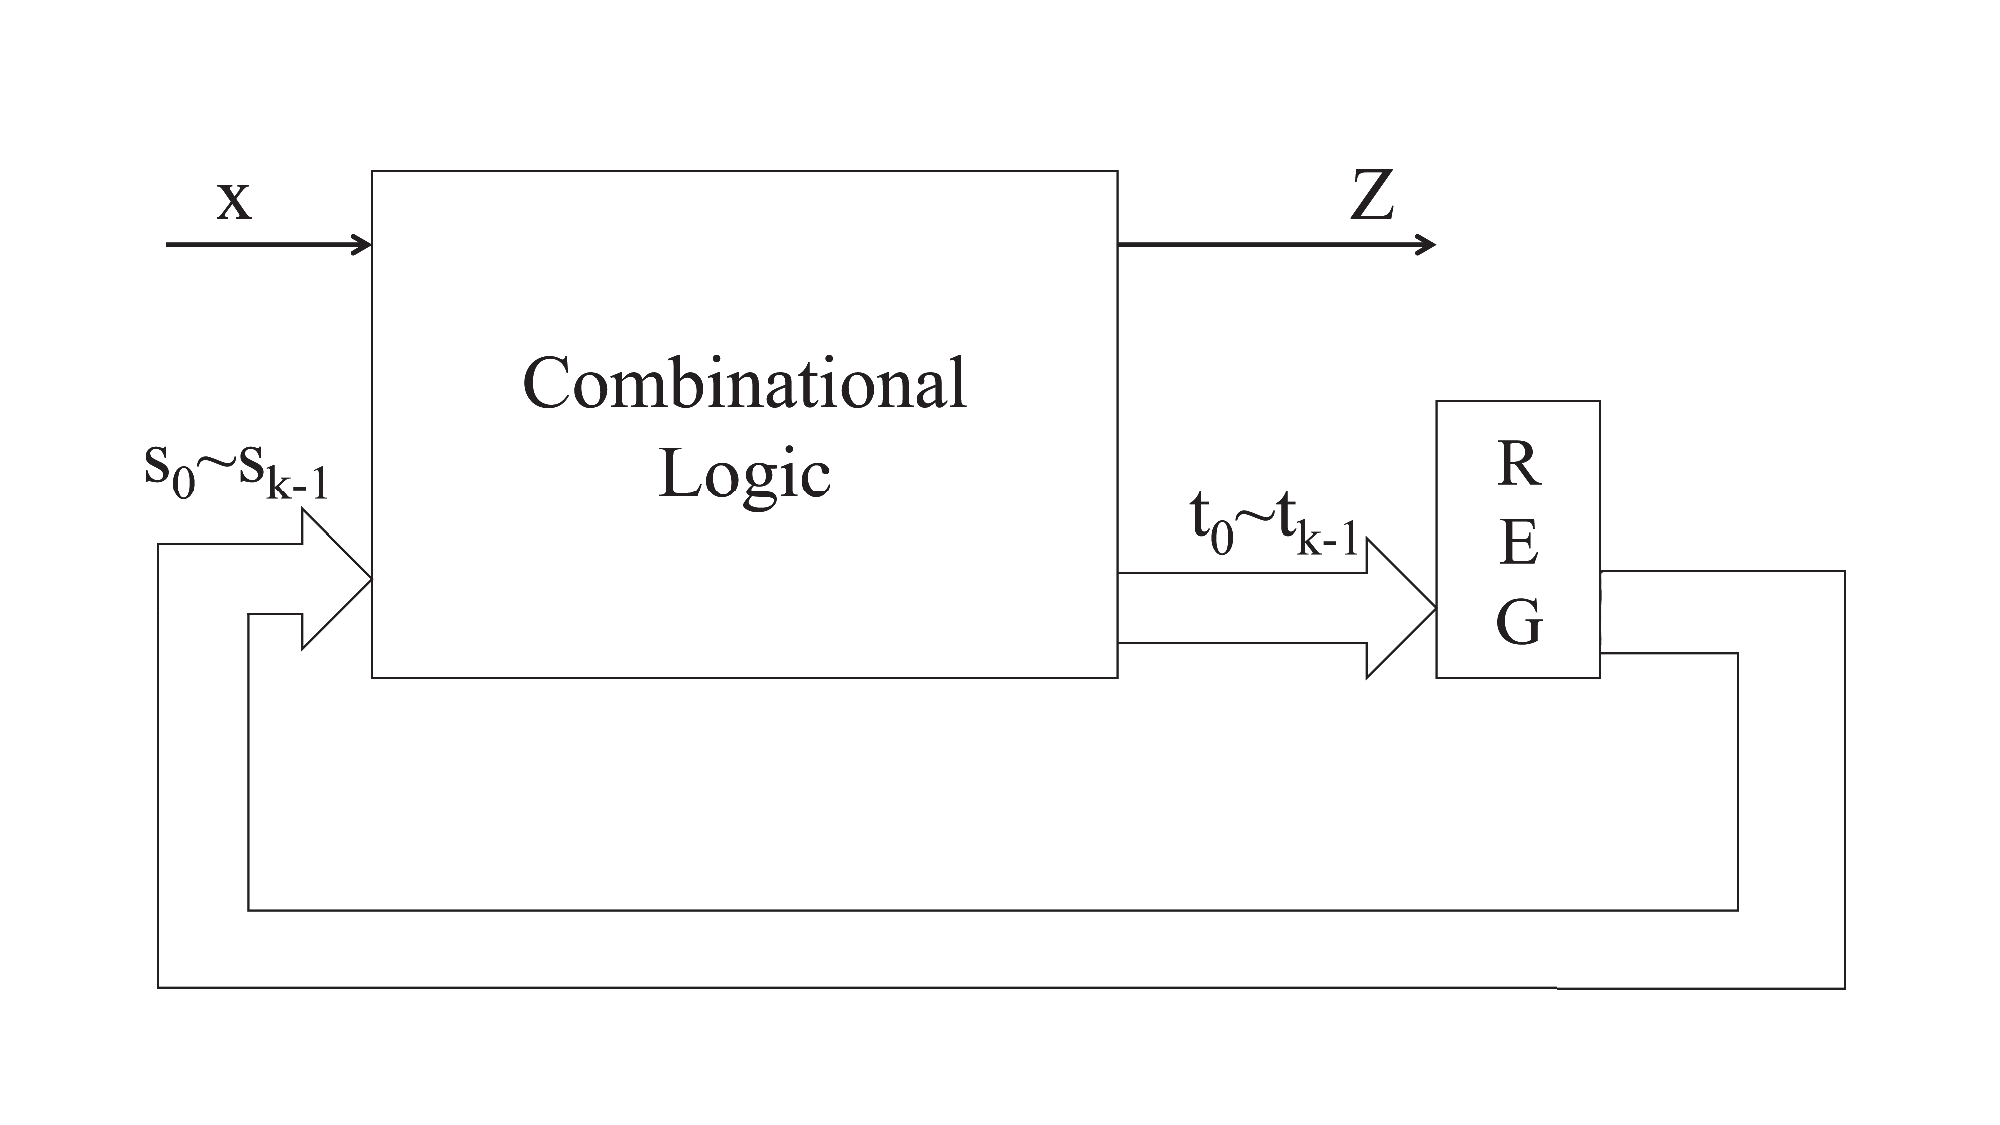
\includegraphics[scale=0.25]{sequential_fig.eps}
}
\end{figure}

\begin{itemize}
\item Primary input(s): x, primary output(s): Z
\item Pseudo inputs: $\{s_0, s_1, \dots, s_{k-1}\}$
\item Pseudo outputs: $\{t_0, t_1, \dots, t_{k-1}\}$
\end{itemize}
\end{frame}
%%%%%%%%%%%%%%%%%%%%%%%%%%%%%%%%%%%%%%%%%%%%%%%%%%%%%
\begin{frame}{\large{A FSM Example}}
\begin{columns}

\begin{column}{0.3\textwidth}

\begin{figure}[hbt]
\centerline{
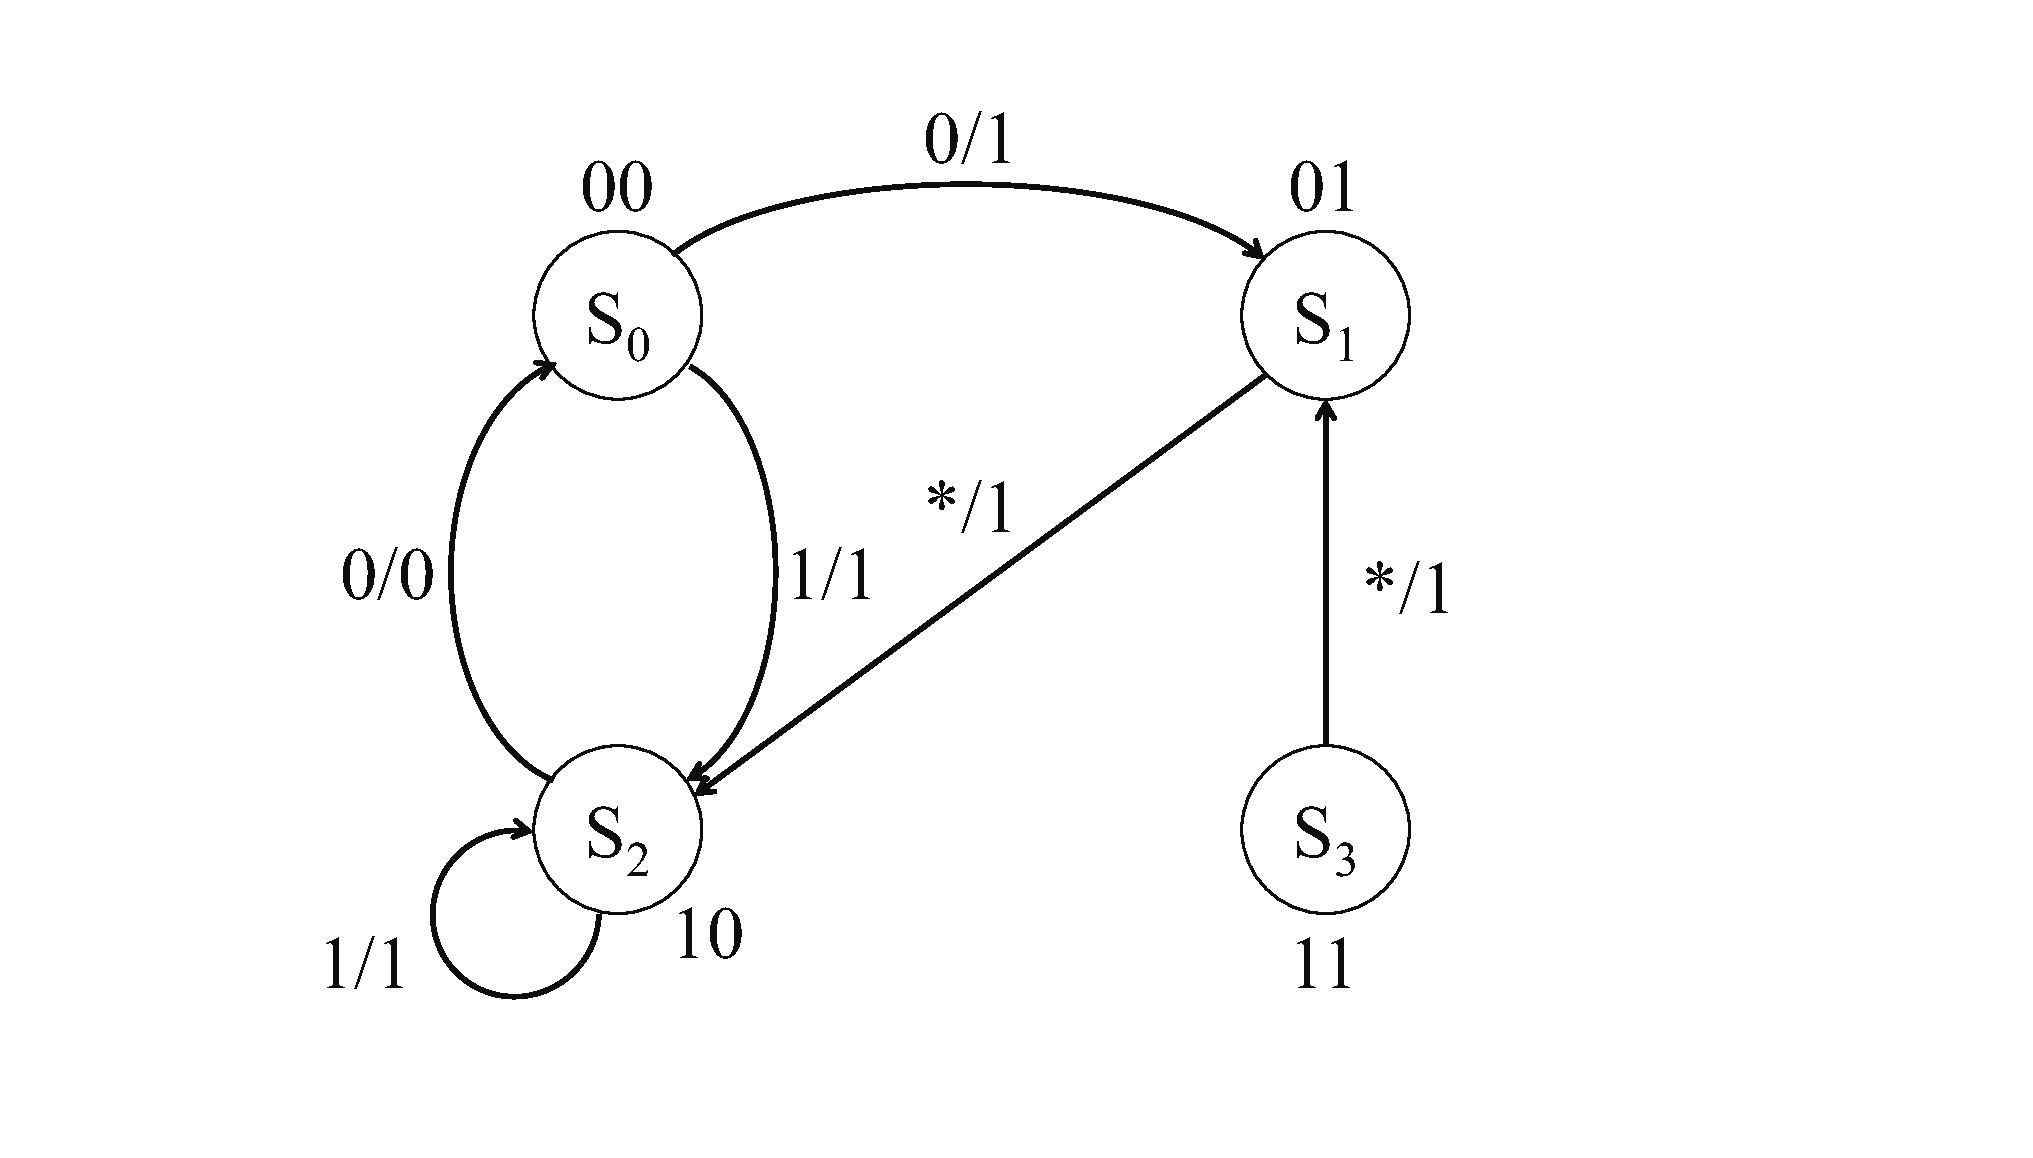
\includegraphics[scale=0.25]{stg_fig.ps}
}
\caption{State Transition Graph}
\end{figure}

\end{column}
%%\end{minipage} \hfill \begin{minipage}[h]{3in}

\begin{column}{0.3\textwidth}
\begin{figure}[hbt]
\centerline{
\includegraphics[scale=0.2]{fsm_fig.eps}
}
\caption{Corresponding Gate-level Circuit}
\end{figure}
\end{column}

\end{columns}
\end{frame}

%%%%%%%%%%%%%%%%%%%%%%%%%%%%%%%%%%%%%%%%%%%%%%%%%%%%%
\begin{frame}{\large{Breadth-First Traversal Algorithm}}
\begin{algorithm}[H]
\SetAlgoNoLine
 \KwIn{Transition functions $\Delta$, initial state $S^0$}
  $from^0 = reached = S^0$\;
  \Repeat{$new^i == 0$}
  {
  	$i \gets i + 1$\;
	$to^i \gets$Img$(\Delta, from^{i-1})$\;
	$new^i \gets to^i \cap \overline{reached}$\;
  	$reached \gets reached \cup new^i$\;
	$from^i \gets new^i$\;
  }
\Return{$reached$}
\caption {Breadth-first Traversal Algorithm}\label{alg:BFS}
\end{algorithm}
\vspace{5mm}
Image function, states intersection, union and complement in this algorithm
will be implemented in computer algebra and algebraic geometry.
\end{frame}
%%%%%%%%%%%%%%%%%%%%%%%%%%%%%%%%%%%%%%%%%%%%%%%%%%%%%%

\begin{frame}{\large{Implement Image Function in Computer Algebra}}
\begin{itemize}
\item State variables (word-level) $S, T$ and sets of states such as
$from^i, to^i$ can always be represented as varieties of ideals.
\item Boolean operators can always be converted to operations in $\mathbb F_2$
\begin{table}
\centering
\begin{tabular}{|c|c|} \hline
Boolean operator & operation in $\mathbb{F}_{2}$\\ \hline
$\overline{a}$ & $1 + a$\\ \hline
$a\ and\ b$ & $ab$\\ \hline
$a\ or\ b$ & $a + b + ab$\\ \hline
$a \oplus b$ & $a + b$\\
\hline\end{tabular}
\caption{Some Boolean operators and corresponding operations in $\mathbb{F}_{2}$}
\label{table:booltogalois_op}
\end{table}
\item An \emph{elimination ideal} can be built from circuit gates, pseudo input/output
word definition and vanishing polynomials
\end{itemize}
\end{frame}

%%%%%%%%%%%%%%%%%%%%%%%%%%%%%%%%%%%%%%%%%%%%%%%%%%%%%%%%%%%
\begin{frame}{\large{Implement Image Function in Computer Algebra(2)}}
Elimination ideal to model Image function for example STG:
\begin{itemize}
\item Transition functions (bit-level): \\ \vspace{-5mm}
\begin{displaymath}
\begin{array}{ll}
f_1:& t_0 - (\overline{x}\ and\ \overline{s_0}\ and\ \overline{s_1})\ or\ (s_0\ and\ s_1) \\
f_2:& t_1 - (\overline{s_0}\ and\ x)\ or\ (s_0\ and\ \overline{s_1})\
\end{array}
\end{displaymath}
\item Word variable definitions:\\ \vspace{-5mm}
\begin{displaymath}
\begin{array}{ll}
f_3:& S - s_0 - s_1\alpha \\
f_4:& T - t_0 - t_1\alpha
\end{array}
\end{displaymath}
\item Vanishing polynomials: $f_6: x^2 - x; f_7: t_0^2 - t_0; f_8: t_1^2 - t_1; f_9: S^4 - S; f_{10}: s_0^2 - s_0;
f_{11}: s_1^2 - s_1; f_{12}: T^4 - T$
\end{itemize}
Add the current state (for example, add initial states in first iteration $f_5: S$), compute Gr\"obner basis
for ideal $J = \langle f_1,\dots, f_{12}\rangle$ under elimination term order $$intermediate\ bit\text{-}level\ signals >\ bit\text{-}level\ primary\ inputs/outputs >\ S >\ T$$
  result will include a univariate polynomial about \emph{next states} $T$.
\end{frame}

%%%%%%%%%%%%%%%%%%%%%%%%%%%%%%%%%%%%%%%%%%%%%%%%%%%%%%%%%%%
\begin{frame}{\large{Algebraic Geometry Concepts}}
\begin{Definition}
\label{def:sum}
({\bf Sum of Ideals}) If $I$ and $J$ are ideals in $k[x_1, \dots, x_n]$, then the 
{\bf sum} of $I$ and $J$, denoted by $I + J$, is the set
  \begin{equation}
  I + J = \{f + g\ |\ f \in I \ and\  g \in J\}.\nonumber
  \end{equation}
Furthermore, if $I = \langle f_1, \dots, f_r\rangle$ and 
$J = \langle g_1, \dots, g_s\rangle$, then 
$I + J = \langle f_1, \dots, f_r, g_1, \dots, g_s\rangle$.
\end{Definition}
\begin{Definition}
\label{def:prod}
({\bf Product of Ideals}) If $I$ and $J$ are ideals in $k[x_1, \dots, x_n]$, then the
{\bf product} of $I$ and $J$, denoted by $I \cdot J$, is defined to be the ideal generated 
by all polynomials $f \cdot g$ where $f \in I$ and $g \in J$. Furthermore, let
$I = \langle f_1, \dots, f_r\rangle$ and $J = \langle g_1, \dots, g_s\rangle$, then
  \begin{equation}
  I \cdot J = \langle f_ig_j\ |\ 1 \leq i \leq r, 1 \leq j \leq s\rangle .\nonumber
  \end{equation}
\end{Definition}
\end{frame}

%%%%%%%%%%%%%%%%%%%%%%%%%%%%%%%%%%%%%%%%%%%%%%%%%%%%%%%%%%%%%
\begin{frame}{\large{Algebraic Geometry Concepts(2)}}
\begin{Definition}
({\bf Quotient of Ideals}) If $I$ and $J$ are ideals in $k[x_1, \dots, x_n]$, then $I:J$
is the set
  \begin{equation}
  \{f \in k[x_1, \dots, x_n]\ |\ f\cdot g \in I, \forall g \in J\}\nonumber
  \end{equation}
and is called the {\bf ideal quotient} of $I$ by $J$.
\end{Definition}
\vspace{5mm}
Concepts are adopted by following theorems:
\begin{Theorem}
\label{thm:unionintersect}
If $I$ and $J$ are ideals in $k[x_1, \dots, x_n]$, then ${\bf V}(I + J) = {\bf V}(I)
\bigcap {\bf V}(J)$ and ${\bf V}(I \cdot J) = {\bf V}(I) \bigcup {\bf V}(J)$.
\end{Theorem}
\begin{Theorem}
\label{thm:quotient}
If $I, J$ are ideals with only one generator, then ${\bf V}(I:J) ={\bf V}(I) - {\bf V}(J)$.
\end{Theorem}
\end{frame}

%%%%%%%%%%%%%%%%%%%%%%%%%%%%%%%%%%%%%%%%%%%%%%%%%%%%%%%%%%%%%
\begin{frame}{\large{New Traversal Algorithm using Algebraic Geometry}}

\begin{algorithm}[H]
\SetAlgoNoLine
 \KwIn{Input-output circuit characteristic polynomial ideal $I_{ckt}$, initial state polynomial $\mathcal F(S)$}

  $from^0 = reached = \mathcal F(S)$\;
  \Repeat{$new^i == 1$}
  {
  	$i \gets i + 1$\;
	$to^i \gets$GB w/ elimination term order$\langle I_{ckt}, from^{i-1}\rangle$\;
	$new^i \gets $generator of $\langle to^i\rangle + (\langle T^4-T\rangle:\langle reached\rangle)$\;
  	$reached \gets $generator of $\langle reached\rangle \cdot \langle new^i\rangle$\;
	$from^i \gets new^i(S\setminus T)$\;
  }
\Return{$reached$}
\caption {Algebraic Geometry based Traversal Algorithm}\label{alg:modified}
\end{algorithm}
\end{frame}

%%%%%%%%%%%%%%%%%%%%%%%%%%%%%%%%%%%%%%%%%%%%%%%%%%%%%%%%%%%%%%%%
\begin{frame}{\large{Example Executing New Traversal Algorithm}}
State encodings are mapped to varieties of ideals, e.g.:
$$\{00,01\} \to \{0,1\} = V_{\mathbb F_{2^2}}(\langle T^2 + T\rangle)$$
$$\{01,10,11\} \to \{1,\alpha, 1+\alpha\} = V_{\mathbb F_{2^2}}(\langle T^3 + 1\rangle)$$
\begin{itemize}
\item Iteration 0: Assume initial state is $\{00\} \to \{0\}$
\item Iteration 1: $reached = from^0 = 0 = V_{\mathbb F_{2^2}}(\langle S\rangle), to^1 = \{1,\alpha\} = V_{\mathbb F_{2^2}}(\langle T^2+(1+\alpha)T+\alpha\rangle), 
new^1 = to^1, reached = \{0,1,\alpha\} = V_{\mathbb F_{2^2}}(\langle T^3+(1+\alpha)T^2+\alpha T\rangle)$
\item Iteration 2: $from^1 = new^1(S\setminus T) = \{1,\alpha\} = V_{\mathbb F_{2^2}}(\langle S^2+(1+\alpha)S+\alpha\rangle), to^2 = \{0,\alpha\}
= V_{\mathbb F_{2^2}}(\langle T^2+\alpha T\rangle),new^2 = 1, \textbf{Terminate}$
\item Return $reached = \{0,1,\alpha\} = V_{\mathbb F_{2^2}}(\langle T^3+(1+\alpha)T^2+\alpha T\rangle)$
\end{itemize}
\end{frame}

%%%%%%%%%%%%%%%%%%%%%%%%%%%%%%%%%%%%%%%%%%%%%%%%%%%%%%%%%%%%%%%%%%%
\begin{frame}{\large{An Application -- Sequential Galois Arithmetic Circuits Verification}}
\begin{figure}[hbt]
\centerline{
\includegraphics[scale=0.35]{mySMPO.eps}
}
\caption{5-bit Normal Basis Angew's Sequential Multiplier with Parallel Output (SMPO)}
\end{figure}
\end{frame}

%%%%%%%%%%%%%%%%%%%%%%%%%%%%%%%%%%%%%%%%%%%%%%%%%%%%%%%%%%%%%%%%%%%
\begin{frame}{\large{SMPO Protocol}}
\begin{itemize}
\item \textbf{Initial}\ \ $R_0 = R_1 = R_2 = R_3 = R_4 = 0$
\item \textbf{Clock 1}\ \ $R_0 = a_1b_0, R_1 = b_2(a_1 + a_4), R_2 = b_4(a_0 + a_1), R_3 = b_1(a_4 + a_0), 
			R_4 = b_3(a_1 + a_3)$
\item \textbf{Clock 2}\ \ $R_0 = b_3(a_1 + a_3) + a_0b_4, R_1 = a_1b_0 + b_1(a_0 + a_3), R_2 = b_2(a_1 + a_4)
			+ b_3(a_4 + a_0), R_3 = b_4(a_0 + a_1) + b_0(a_3 + a_4), R_4 = b_1(a_4 + a_0) + b_2(a_0 + a_2)$
\item \textbf{$\dots$}
\item \textbf{Clock 5}\ \ $R_0 = c_0, R_1 = c_1, R_2 = c_2, R_3 = c_3, R_4 = c_4$, i.e. $R = A\cdot B$.
\end{itemize}
\end{frame}

%%%%%%%%%%%%%%%%%%%%%%%%%%%%%%%%%%%%%%%%%%%%%%%%%%%%%%%%%%%%%%%%%%%
\begin{frame}{\large{Compose Elimination Ideal for 5-bit SMPO}}
An elimination ideal for the first clock cycle:
\begin{itemize}
\item {\bf Gate descriptions:}
$a_1+a_4+c_1, a_1+a_0+c_2, a_0+a_4+c_3, a_1+a_3+c_4,
		  a_1b_0+r_4+R_0, c_1b_2+r_0+R_1, c_2b_4+r_1+R_2, c_3b_1+r_2+R_3, c_4b_3+r_3+R_4;$
		  
\item {\bf Word-level variables:}
$A+a_0\alpha^5+a_1\alpha^{10}+a_2\alpha^{20}+a_3\alpha^9+a_4\alpha^{18},
		  B+b_0\alpha^5+b_1\alpha^{10}+b_2\alpha^{20}+b_3\alpha^9+b_4\alpha^{18},
		  r+r_0\alpha^5+r_1\alpha^{10}+r_2\alpha^{20}+r_3\alpha^9+r_4\alpha^{18},
		  R+R_0\alpha^5+R_1\alpha^{10}+R_2\alpha^{20}+R_3\alpha^9+R_4\alpha^{18};$
		  
\item {\bf Vanishing polynomials:}
		 $ a_0^2+a_0, a_1^2+a_1, a_2^2+a_2, a_3^2+a_3, a_4^2+a_4,
		  b_0^2+b_0, b_1^2+b_1, b_2^2+b_2, b_3^2+b_3, b_4^2+b_4,
		  r_0^2+r_0, r_1^2+r_1, r_2^2+r_2, r_3^2+r_3, r_4^2+r_4,
		  R_0^2+R_0, R_1^2+R_1, R_2^2+R_2, R_3^2+R_3, R_4^2+R_4,
		  c_1^2+c_1, c_2^2+c_2, c_3^2+c_3, c_4^2+c_4,
		  A^{32}+A, B^{32}+B, r^{32}+r, R^{32}+R;$
		  
\item	{\bf Feedback input:}	  $r_{in}$.
\end{itemize}
\end{frame}

%%%%%%%%%%%%%%%%%%%%%%%%%%%%%%%%%%%%%%%%%%%%%%%%%%%%%%%%%%%%%%%%%%%%
\begin{frame}{\large{Fast Abstraction without GB computation}}
\begin{Definition}
A lexicographic order constrained by following relation $>_{r}$: "circuit variables ordered reverse topologically" $>$ 
"designated word-level output" $>$ "word-level inputs" is called the \emph{Refined Abstraction Term Order (RATO)}.
\end{Definition}
\begin{Example}
The elimination ideal for 5-bit SMPO could be rewritten under RATO:
\begin{align}
&(R_0,R_1,R_2,R_3,R_4)>(r_0,r_1,r_2,r_3,r_4)\nonumber\\&>(c_1,c_2,c_3,c_4,b_0,b_1,b_2,b_3,b_4)\nonumber\\
&>(a_0,a_1,a_2,a_3,a_4)>R>r>(A,B)\nonumber
\end{align}
\end{Example}
\end{frame}

%%%%%%%%%%%%%%%%%%%%%%%%%%%%%%%%%%%%%%%%%%%%%%%%%%%%%%%%%%%%%%%%%%%
\begin{frame}
Under RATO, most polynomials
have relatively prime leading terms/monomials (which means $Spoly \xrightarrow{J+J_0}_{+} 0$) except one pair:
word-level polynomial corresponding to outputs and its leading bit-level variable's gate description polynomial.
\begin{Example}
Candidate pair for 5-bit SMPO is
$(f_w,f_g), f_w = R_0+r_4+b_0\cdot a_1, f_g =R_0\alpha^5+R_1\alpha^{10}+R_2\alpha^{20}+R_3\alpha^9+R_4\alpha^{18} + R$.
Result after reduction is an abstraction:
\begin{align}
&Spoly(f_w,f_g) \xrightarrow{J+J_0}_{+}\nonumber\\
&r_1+(\alpha)r_2+(\alpha^4+\alpha^2)r_3+(\alpha^3+\alpha^2)r_4+(\alpha^3)b_1a_1\nonumber\\
+&(\alpha^4+\alpha^2)b_1a_2+(\alpha^3+\alpha+1)b_1a_3+(\alpha^3+\alpha)b_1a_4+(\alpha+1)b_1A\nonumber\\
+&(\alpha^4+\alpha^2+\alpha)b_2a_1+(\alpha^4+\alpha^3+\alpha^2+\alpha)b_2a_4+(\alpha^3+\alpha^2+1)b_3a_1\nonumber\\
+&(\alpha)b_3a_3+(\alpha^2+\alpha+1)b_4a_1+(\alpha+1)b_4a_2+(\alpha^4+\alpha^2)b_4a_3\nonumber\\
+&(\alpha^4+\alpha^3+\alpha+1)b_4a_4+(\alpha^3+1)b_4A+(\alpha^4+\alpha^3+\alpha^2+1)a_1B\nonumber\\
+&(\alpha^4+\alpha^3+\alpha^2+1)R\nonumber
\end{align}
\end{Example}
\end{frame}

%%%%%%%%%%%%%%%%%%%%%%%%%%%%%%%%%%%%%%%%%%%%%%%%%%%%%%%%%%%%%%%%%%%%
\begin{frame}{\large{Bit-Level Variable Substitution (BLVS)}}
Use Gaussian elimination style approach, eliminate other bit-level variables except for one.
\begin{Example}
{\bf Objective}:\ Abstract polynomial $a_i + \mathcal{G}_i(A)$ from $f_0: a_0\alpha^5+a_1\alpha^{10}+a_2\alpha^{20}+a_3\alpha^9+a_4\alpha^{18}+A$.
Eliminate variable $a_0$ by operation 
\begin{align}
f_1 =& f_0\times \alpha^5 + f_0^2: \nonumber\\
&a_1+(\alpha)a_2+(\alpha^4+\alpha^2)a_3+(\alpha^3+\alpha^2)a_4\nonumber\\
+&(\alpha^4+\alpha^3+\alpha^2+1)A^2+(\alpha^2+\alpha)A\nonumber
\end{align}
Recursively eliminate $a_1$ from $f_1$, $a_2$ from $f_2$, etc. 
\end{Example}
\end{frame}

%%%%%%%%%%%%%%%%%%%%%%%%%%%%%%%%%%%%%%%%%%%%%%%%%%%%%%%%%%%%%%%%%%%%%%
\begin{frame}{\large{Bit-Level Variable Substitution (BLVS) (2)}}
\begin{Example}
For 5-bit SMPO example, the result is
\begin{displaymath}
\left\{
  \begin{array}{lcl}
  a_0 & = & (\alpha+1)A^{16}+(\alpha^4+\alpha^3+\alpha)A^8+(\alpha^3+\alpha^2)A^4\\&&+(\alpha^4+1)A^2+(\alpha^2+1)A\\
  a_1 & = & (\alpha^2+1)A^{16}+(\alpha+1)A^8+(\alpha^4+\alpha^3+\alpha)A^4\\&&+(\alpha^3+\alpha^2)A^2+(\alpha^4+1)A\\
  a_2 & = & (\alpha^4+1)A^{16}+(\alpha^2+1)A^8+(\alpha+1)A^4\\&&+(\alpha^4+\alpha^3+\alpha)A^2+(\alpha^3+\alpha^2)A\\
  a_3 & = & (\alpha^3+\alpha^2)A^{16}+(\alpha^4+1)A^8+(\alpha^2+1)A^4\\&&+(\alpha+1)A^2+(\alpha^4+\alpha^3+\alpha)A\\
  a_4 & = & (\alpha^4+\alpha^3+\alpha)A^{16}+(\alpha^3+\alpha^2)A^8+(\alpha^4+1)A^4\\&&+(\alpha^2+1)A^2+(\alpha+1)A
  \end{array} \right.
\end{displaymath}
\end{Example}
By substitution of bit-level variables in remainder from RATO, get next state abstraction $R+\mathcal F(A,B)$
\end{frame}

%%%%%%%%%%%%%%%%%%%%%%%%%%%%%%%%%%%%%%%%%%%%%%%%%%%%%%%%%%%%%%%%%%%%%%%
\begin{frame}{\large{Results Comparing to SAT/ABC/BDD}}
\begin{table}[H]
\centering
\begin{tabular}{|c||c|c|c|c|} 
\hline
& \multicolumn{4}{|c|}{Word size of the operands $k$-bits}  \\
\hline
Solver & 11 & 18 & 23 & 33 \\
\hline
\hline
Lingeling & 593  & \emph{TO}  & \emph{TO}  & \emph{TO}\\
\hline
\hline
ABC & 6.24 & \emph{TO} & \emph{TO} & \emph{TO}\\
\hline
\hline
BDD & 0.1 & 11.7 & 1002.4 & \emph{TO}  \\
\hline
\end{tabular}
\caption{Runtime for verification of bug-free SMPO circuits over $\Fkk$ for SAT, ABC and BDD based methods. \emph{TO} = timeout of 14 hrs}\label{table:satbdd}  
\end{table}
\end{frame}

%%%%%%%%%%%%%%%%%%%%%%%%%%%%%%%%%%%%%%%%%%%%%%%%%%%%%%%%%%%%%%%%%%%%%%
\begin{frame}{\large{Results from our approach}}
\begin{table}[H]
\centering
\begin{tabular}{|c||c|c|c|c|c|} 
\hline
Operand size $k$ & 36 & 66 & 82 & 89 & 100 \\
\hline
\#variables & 183 & 333 & 413 & 448 & 503\\
\hline
\#polynomials & 2700 & 8910 & 13694 & 16109 & 20300\\
\hline
\#terms & 12996 & 43626 & 67322 & 79299 & 100100 \\
\hline
\hline
Runtime(bug-free) & 113 & 3673 & 15117 & 28986 & 50692 \\
\hline
Runtime(buggy) & 118 & 4320 & 15226 & 31571 & 58861\\
\hline
\end{tabular}
\caption{Runtime (given in seconds) for verification of bug-free and buggy Angew's SMPO circuits over $\Fkk$ using our approach}\label{table:SMPO}  
\end{table}
\end{frame}

\end{document}
